
\documentclass[12pt]{article}

\title{A spatial stochastic discount factor estimator for private equity funds}

\author{
	Christian Tausch  \\
	AssetMetrix GmbH  \\
	Theresienh\"{o}he 13, D-80339 Munich \\
	christian.tausch@quant-unit.com \\
	% \and 
	}

\date{\today}



% Packages
\usepackage{amssymb}
\usepackage{amsmath}
\usepackage{natbib}
\usepackage{graphics}
% use smaller margins
\usepackage[margin=1.0in]{geometry} % 1.25in
% use double spacing
\usepackage{setspace}
\usepackage{amsthm}
\usepackage{url}
\usepackage[outdir=./]{epstopdf}


\newtheorem{prop}{Proposition}
\newtheorem{assume}{Assumption}


\begin{document}

\maketitle


\section*{Keywords}
Stochastic discount factor, Private equity fund, Fund level data set


\section*{Acknowledgements}
I thank Hsin-Chih Ma, Stefan Mittnik, Daniel Schalk, and all participants of the LMU econometrics research seminar SS 2019 for helpful discussions and support.


\section*{Declaration of interest}
The author reports no conflict of interest. 
The author alone is responsible for the content and writing of the paper.


\newpage
%\doublespacing

\begin{center} 
\section*{A spatial stochastic discount factor estimator for private equity funds}
\end{center}



\begin{abstract}
This paper proposes a stochastic discount factor estimation methodology suited for private equity fund-level cash flow data.
The asymptotic inference framework for our least-mean-distance estimator draws on a spatial notion, i.e., the idea that the economic distance between distinct private equity funds can be measured.
\end{abstract}

%% main text
\section{Introduction}
Do investments in private equity funds offer abnormal returns to fund investors when risk-adjusted to/for public market factors?
Currently, a popular approach to answer this question is to evaluate private equity fund cash flows by Stochastic Discount Factor (SDF) models that draw on public market return covariates.
The basic idea for SDF model estimation is that the sum of all discounted fund net cash flows is zero when the true SDF is applied.
Unfortunately, there is no conclusion about the best methodology to estimate these SDF models, as a variety of proposal coexists in the academic private equity fund literature \citep{DLP12,KN16,ACGP18,GSW19}.


Especially our conclusions from the \cite{DLP12} and \cite{KN16} approaches lead us to suggest a new least-mean-distance estimator for SDF models that is applicable to private equity fund-level cash flow data.
On the one hand, we provide asymptotic inference formulations that rely on the concept of spatial (near-epoch) dependency between funds comparable to \cite{KN16}.
In this context, it is paramount to quantify the economic distance between funds by a measure like absolute vintage year difference or cash flow overlap\footnote{However, this economic inter-fund distance refers NOT to the term least-mean-distance estimator.}.
On the other hand, our least-mean-distance estimator can be regarded as generalization of the \cite{DLP12} methodology, where we provide the asymptotic inference framework that was missing in the original paper.
In contrast to \cite{DLP12}, we explicitly do not require the pooling of private equity fund cash flows to form vintage year portfolios.
The increased number of cross-sectional units (in a fundwise approach) in turn decreases the asymptotic variance of coefficient estimates compared to the case when just a small number of vintage year portfolios is available.

In the empirical application of our new estimator, we estimate an exponentially affine SDF model that can draw on the five return factors associated with the $q^5$ investment factor model recently proposed by \cite{HXZ20}.
We calculate asymptotic standard errors and a Wald test statistic for the model coefficients.
Moreover, we assess the small-sample variance of coefficient estimates and the out-of-sample performance of the different SDF models by $hv$-block cross validation which accounts for the inter-vintage-year dependence of private equity funds \citep{R00}.

The paper is structured as follows. 
Section \ref{sec:Methodology} introduces our fundwise least-mean-distance estimator and its corresponding asymptotic inference framework.
Section \ref{sec:empirical_estimation} applies the method to estimate $q^5$-investment-factor SDFs for various private equity fund types.
Section \ref{sec:conclusion} concludes.


\section{Methodology}
\label{sec:Methodology}

\subsection{Fundwise least-mean-distance estimator}

Let fund $i=1,2,\dots,n$ be characterized by its (net) cash flows ${CF}_{t,i}$ and its net asset values ${NAV}_{t,i}$ with discrete time index $t=1,2,\dots,T$.
The data generating processes for $CF$ and $NAV$ are left unspecified.
The stochastic discount factor $\Psi_{t,\tau}$ can be used to calculate the time-$\tau$ present value $P_{t,\tau,i}$ of a time-$t$ cash flow of any given PE fund $i$
\begin{equation}
\label{eq:price}
P_{t,\tau,i} = \Psi_{t,\tau} \cdot CF_{t,i}
\end{equation}
As SDFs are commonly parameterized by a vector $\theta \in \mathbb{R}^p$, i.e., $\Psi_{t,\tau} \equiv \Psi_{t,\tau} (\theta)$, our goal is to find an estimation method for the optimal $\theta$.
For each fund $i$ and all points $\tau$ within a common fund lifetime, the pricing error $\epsilon_{\tau,i}$ of all fund cash flows is calculated as
\begin{equation}
\label{eq:pricing_error}
\epsilon_{\tau,i} = \sum_{t=1}^T P_{t,\tau,i} 
\qquad \forall \quad \tau,i
\end{equation}
We define the $w$-weighted $\tau$-average fund pricing error as
\begin{equation}
\label{eq:average_pricing_error}
\bar{\epsilon}_{i} =
w_{i} \cdot
\frac{1}{\mathrm{card}( \mathcal{T}_{i})}
\sum_{\tau \in \mathcal{T}_{i}}
\epsilon_{\tau,i}
\qquad \forall \quad i
\end{equation}
where $\mathcal{T}_i$ gives the set of relevant present value times $\tau$ for fund $i$, which can be thought of as all quarterly/yearly dates within the usual fund lifetime of ten to fifteen years.
Each fund $i$ is characterized by its vintage year which can be expressed by $v_{i}=\min(\mathcal{T}_i) \in 1,2,\dots,V$, where $V$ denotes the maximum vintage year used in a given data set.
Here we implicitly assume that $\mathcal{T}_i$ always contains at least the fund's starting date.
Finally, the scalar weighting factor $w_i$ can be (i) one divided by the fund's invested capital for equal weighting of funds, (ii) one divided by the vintage year sum of invested capital for vintage year weighting, (iii) the scalar one for fund-size weighting, or (iv) some macroeconomic deflator.

Our least-mean-distance estimator minimizes the average loss of $\bar{\epsilon}$
\begin{equation}
\label{eq:estimator}
\hat{\theta} = 
\mathrm{arg \ min}_{\theta \in \Theta}
\enspace
S_n(\theta)
\quad
\mathrm{with}
\quad
S_n(\theta) = 
\frac{1}{n}
\sum_{i=1}^n
L \left( \bar{\epsilon}_{i} \right) 
\end{equation}
where $L$ denotes a loss function, e.g., $L(x)=(x-0)^2$.
Throughout the paper, the weighted average fund pricing error $\bar{\epsilon} \equiv \bar{\epsilon}(\theta)$ is regarded as nonlinear random function of the SDF parameter $\theta$.


\subsection{Asymptotic framework}
\label{sec:asymptotic_framework}

\subsubsection{Vintage year asymptotics}
We employ a spatial framework, where we assume that the (spatial, i.e., economic) distance between cross-sectional units, i.e., private equity funds, can be measured in quantitative way.
Here asymptotic results are derived for the case when the number of funds goes to infinity $n \to \infty$.
However, to expose our SDF to enough distinct covariate realizations (economic conditions), identification of model parameters requires a sufficient number of funds from different vintage years in the fund-level data set used for model estimation \citep{DLP12,KN16}.
\begin{assume}
	(i) The number of vintage years $V \to \infty$ as $n \to \infty$.
	(ii) The number of funds per vintage year is bounded by some positive constant.
	(iii) The maximal fund lifetime is also bounded by a positive constant.
	(iv) The economic distance between fund $i$ and $j$ is measured by the vintage year difference $d_{i,j}=v_i - v_j$.
\end{assume}

\subsubsection{Law of large numbers}
The global moment condition underlying our estimation approach is that the ($i$-unconditional) expected value of $\bar{\epsilon}$ shall be zero, if we use the optimal SDF parameter $\theta_0$. 
This also means, instead of applying a time-series law of large numbers, we rely on a spatial (cross-sectional) law of large numbers, but acknowledge the statistical dependence of  pricing errors with respect to vintage year differences between funds.
\cite{JP12} develop an asymptotic inference framework for near-epoch dependent spatial processes that is instructive for our setting.

\begin{assume}
	The (i) time-trend and (ii) dependence structure of $\bar{\epsilon}$ shall allow
	\[
	n^{-1} \sum_{i=1}^n \overline{\epsilon}_i \overset{a.s.}\to E[\bar{\epsilon}]
	\quad {as} \quad V,n \to \infty
	\]
	Specifically, the process $\overline{\epsilon}$ is spatial near-epoch dependent with respect to fund vintage years \citep{JP12}, i.e., two funds with distance $d_{i,j}>D$ are assumed to be independent.
\end{assume}
To satisfy the time trend part (i) of this law of large number assumption, the weighting factor $w$, introduced in equation \ref{eq:average_pricing_error}, can be used to make $\bar{\epsilon}$ stationary.
Spatial near-epoch dependence with respect to fund vintage years formalizes the idea that two funds with a small absolute vintage year difference are supposed to be dependent (due to being exposed to the same macroeconomic condition), whereas two funds with a very large absolute vintage year difference can be assumed to be independent.
In our framework, spatial distance is considered as economic distance between funds (represented by $\bar{\epsilon}$); our spatial space is thus of dimension one.

\subsubsection{Consistency}
The estimator $\hat{\theta}$ shall converge in probability to the true parameter value $\theta_0$ as the number of distinct vintage years in our data set goes to infinity.
Multiple funds for a specific vintage year are not necessarily required and are thus considered as additional, stabilizing moment conditions.

\begin{assume}
 Consistency of $\hat{\theta}$ requires $\hat{\theta} \overset{p}{\to} \theta_0$ as $V,n \to \infty$.
 Thus $E[\bar{\epsilon}]=0$ if and only if $\theta=\theta_0$.
 The parameter space is compact $\theta \in \Theta$.
\end{assume}
Compactness of $\Theta$ can be assured by lower and upper bounds for all parameters that can be justified by economic reasoning in our case, e.g., a market beta factor of ten seems implausible for PE funds because of the implied risk and return expectations.

\subsubsection{Central limit theorem}
To assess the significance of our parameter estimates, we want to describe the asymptotic distribution of the parameter vector as a normal distribution.

\begin{assume}
	$\sqrt{n}(\hat{\theta} - \theta_0) \overset{d}{\to} \mathcal{N}(0,\mathbf{\Sigma})$ as $V,n \to \infty$ with covariance matrix $\mathbf{\Sigma}$.
\end{assume}

\subsection{Asymptotic inference}
\label{sec:asymptotic_inference}

In the general (time-series) near-epoch-dependent least-mean-distance literature, $\mathbf{\Sigma}$ can be characterized according to \citet[Theorem 11.2.b, Theorem H.1]{PP97}:
\[
\mathbf{\Sigma} = C^{-1} \Delta (C^{-1})^\top
\]
with expected hessian matrix converging to $C$ as $V,n \to \infty$
\[
E 
\left(
\nabla_{\theta \theta} S_n
\right)
\to C
\]
and the expected covariance matrix of gradients converging to $\Delta$ as $V,n \to \infty$
\[
n E 
\left[
\nabla_{\theta} S_n
(\nabla_{\theta} S_n)^\top
\right]
\to \Delta
\]
Here, the gradient vector $\nabla_{\theta} S_n$ is denoted as column vector.
We define the corresponding finite sample estimators analogously to \citet[Chapters 12, 13.1]{PP97} and numerically approximate the first and second derivatives by finite differences. $\hat{C}$ is relatively straightforward
\[
\hat{C} = \frac{1}{n} \sum_{i=1}^n \nabla_{\theta \theta} L \left( \epsilon_i \right)
\]
Due to the (spatial near-epoch) dependence, the intricate part is to consistently estimate $\hat{\Delta}$ by a Spatial Heteroskedasticity and Autocorrelation Consistent (SHAC) covariance matrix estimator \cite[equation 2]{KS11}
\begin{equation}
\label{eq:hac}
\hat{\Delta} = \frac{1}{n} \sum_{i=1}^n \sum_{j=1}^n
k_{i,j}
\left[
\nabla_{\theta} L \left( \epsilon_i \right)
\left(
\nabla_{\theta} L \left( \epsilon_j \right)
\right)^\top
\right]
\end{equation}
We define the kernel weight $k$ as
\[
k_{i,j} \equiv K \left( \frac{d_{i,j}}{b_n} \right)
\]
with kernel function $K: \mathbb{R} \to [0,1]$ satisfies $K(0)=1$, $K(x)=K(-x)$, $\int_{-\infty}^{\infty} K^2(x) dx < \infty$, and $K(\cdot)$ continuous at zero and at all but a finite number of other points.
A common choice is the Bartlett kernel $K_{BT}(x)= \max(0, 1-|x|)$; see equation 2.7 in \cite{A91} for other popular kernel choices.
This means absolute vintage year differences larger than the bandwidth (or truncation) parameter $b_n=D$ are considered independent and are thus excluded from the $\hat{\Delta}$ estimation formula.

In large samples, the parameter standard error vector can thus be estimated by
\[
\mathrm{SE}(\hat{\theta}) = 
\sqrt{
	\mathrm{diag} \left[
	n^{-\frac{1}{2}}
	\hat{C}^{-1} \hat{\Delta} (\hat{C}^{-1})^\top
	(n^{-\frac{1}{2}})^\top
	\right] 
}
=
\sqrt{
	\mathrm{diag} \left[
	\frac{\hat{C}^{-1} \hat{\Delta} (\hat{C}^{-1})^\top}{n}
	\right] 
}
\]
The Wald test statistic for linear hypotheses $H_0: R \theta = r$ and $H_1: R \theta \neq r$ is constructed as
\[
W = 
(R \hat{\theta} - r)^\top
\left[
R
\frac{\hat{C}^{-1} \hat{\Delta} (\hat{C}^{-1})^\top}{n}
R^\top
\right]^{-1}
(R \hat{\theta} - r)
\stackrel{H_0}{\sim}
\chi_q^2
\]
where $\hat{\theta}$ is the $p \times 1$ parameter vector, $R$ is a $q \times p$ matrix, and $r$ is a $q \times 1$ vector.
Usually, we select $R$ as $p \times p$ identity matrix, and $r$ as $p \times 1$ vector (e.g., of zeros).
Under the null hypothesis, $W$ is chi-squared distributed with $q$ degrees of freedom. As large values of $W$ indicate the rejection of $H_0$, the corresponding p-value is calculated as $1 - F_{\chi_q^2}(W)$ where $F_{\chi_q^2}$ is the cumulative distribution function of a chi-squared random variable with $q$ degrees of freedom.

However, in view of the limited amount of available private equity data (typically the oldest vintages start in the 1980s), asymptotic characterizations of $\mathbf{\Sigma}$ and $\mathrm{SE}(\hat{\theta})$ are of limited importance. 
In empirical applications, the small sample behavior of an estimation method for private equity data is more relevant than its asymptotic theory.
Moreover, the standard asymptotic distribution associated with an estimator is generally not valid for post-model-selection inference, i.e., if a model selection procedure is applied to find the best model from a collection of competitors \citep{LP05}.


\subsection{Comparison to other approaches}

The estimator in equation \ref{eq:estimator} exhibits a cross-sectional nature, since it sums over all funds rather than constructing vintage year based time-series.
This means, we intentionally opt against a framework compatible with classical, time-series GMM that requires the construction of stationary, ergodic time-series of moment conditions \citep{H82,H12}.
These time-series (of random functions) are used to empirically estimate the expected value of pricing errors in equation \ref{eq:pricing_error}.
The stationarity requirement of classical time-series GMM restrict us with respect to (i) more elaborate weighting-schemes for $w$, like fund-size weighting, and (ii) the usage of fund cash flows from non-realized vintages.

In contrast to our approach, the closely related method of \cite{DLP12} forms vintage year portfolios instead of using individual fund moments.
Further, they discount all fund cash flows just to the first cash flow date (like in a classical net present value calculation) and we additionally average over all dates within $W_{i}$ to alleviate the exploding alpha issue mentioned in \cite{DLP12}.
Although \cite{DLP12} describe their estimator as one-step GMM approach, it can be regarded very closely related to our least-mean-distance estimator.
Especially, the asymptotic assumptions from subsection \ref{sec:asymptotic_framework} shall be likewise apply to their setting.
Due to the fundwise nature of our approach it is more stable but slower than the vintage year pooling conducted in \cite{DLP12}.
This stability results in smaller asymptotic standard errors for the coefficients.

Similar to our ansatz, \cite{KN16} draw on a spatial framework to handle cross-sectional dependence between funds \citep{C99}.
However, they ultimately utilize a classical GMM estimator, thus a time-series law of large numbers.
To obtain their Generalized Public Market Equivalent (GPME) metric they opt for pricing public market cash flows that shall replicate PE funds instead of directly pricing the observed fund cash flows.
Time-series GMM estimators always bear the risk of under-identification, if the corresponding time series are constructed by pooling all fund cash flows from a given fund type, since you end up with just one moment condition per fund type.


\section{Empirical estimation}
\label{sec:empirical_estimation}

\subsection{Data}

We use the Preqin cash flow data set as of 26th February 2020.
We pool all regions and analyze the following fund types (using the Preqin asset class classification):
PE ("Private Equity"; 2474 distinct funds in data set),
VC ("Venture Capital"; 985),
RE ("Real Estate"; 810),
PD ("Private Debt"; 488),
INF ("Infrastructure", 174), 
NATRES ("Natural Resources", 167).
%MEZZ ("Mezzanine"; 147),
%DD ("Special Situations", "Distressed Debt"; 60+153),
%BO ("Growth", "Buyout"; 265+1251),
%FOF ("Fund of Funds"; 589),
%SEC ("Secondaries"; 131).
For these fund types we extract all (i) equal-weighted and (ii) fund-size-weighted cash flow series.
For non-liquidated funds we treat the latest net asset value as final cash flow.
We explicitly refrain from excluding the most recent vintage years.

The public market factors that enter our SDF draw on the US data set of the recently popularized $q^5$ investment factor model sourced from \url{http://global-q.org/factors.html} \citep{HXZ15,HXZ20}. 
Their five factor model includes: MKT the market excess return, ME the size factor, IA the investment factor, ROE the return on equity factor, and EG the expected growth factor.


\subsection{Model and estimator specifications}
\label{sec:model_selection}

We use the exponential affine SDF analogously to \cite{KN16}
\begin{equation}
\label{eq:SDF}
\Psi_{t,\tau} (\theta) = 
\exp
\left[
-
\sum_{h=\tau}^{t} \left( 1 + r_f + \sum_{j \in J} \theta_{j,h} \cdot F_{j,h} \right)
\right]
\end{equation}
with risk-free return $r_f$ and zero-net-investment portfolio returns $F_j$.
To avoid overfitting, we just test five simple SDF models that contain \{MKT\} alone or \{MKT\} plus \{ME or IA or ROE or EG\}.
We test two different sets for $\mathcal{T}_i$: they include all quarterly $\tau$ horizons smaller than $\{40, 60\}$ quarters, respectively.
In equation \ref{eq:estimator}, we use the quadratic loss function $L(x)=x^2$.

To assess the parameter significance, we compute the asymptotic standard errors as outlined in subsection \ref{sec:asymptotic_inference}.
Moreover, we perform a Wald test for the null hypothesis of a MKT coefficient of one and zeros for the other coefficients (ME, IA, ROE, EG).
The Bartlett kernel's bandwidth $b_n=D$ is selected as 12 years, i.e., funds with absolute vintage year differences larger than 12 years are assumed to be independent.

Additionally, we want to test the finite - or more honestly small - sample parameter significance and the out-of-sample performance of our SDF models.
Here we rely on $hv$-block cross validation to account for the dependency in our data set introduced by overlapping fund cash flows for funds from adjacent vintage years \citep{R00}. 
Therefore, we form three partitions for several vintage year groups. 
As larger validation sets are preferred for model selection, the validation set ($v$-block) always contains funds of three neighboring vintage years (e.g. 2000, 2001, 2002). 
To reduce the dependency between training and validation set, we remove all funds from three-year-adjacent vintage years, i.e., the $h$-block (e.g. 1997, 1998, 1999, 2003, 2004, 2005). 
Funds from the remaining vintage years enter the training set and are thus used for model estimation (e.g. 1985-1996, 2006-2019).
We apply ten-fold cross validation using the ten validation sets described in table \ref{tab:hv_block_cv}.

\begin{table}[ht]
	\centering
	\begin{tabular}{lllll}
		\hline
		training.before & h.block.before & validation & h.block.after & training.after \\ 
		\hline
		start-1984 & 1985,1986,1987 & 1988,1989,1990 & 1991,1992,1993 & 1994-end \\ 
		start-1987 & 1988,1989,1990 & 1991,1992,1993 & 1994,1995,1996 & 1997-end \\ 
		start-1990 & 1991,1992,1993 & 1994,1995,1996 & 1997,1998,1999 & 2000-end \\ 
		start-1993 & 1994,1995,1996 & 1997,1998,1999 & 2000,2001,2002 & 2003-end \\ 
		start-1996 & 1997,1998,1999 & 2000,2001,2002 & 2003,2004,2005 & 2006-end \\ 
		start-1999 & 2000,2001,2002 & 2003,2004,2005 & 2006,2007,2008 & 2009-end \\ 
		start-2002 & 2003,2004,2005 & 2006,2007,2008 & 2009,2010,2011 & 2012-end \\ 
		start-2005 & 2006,2007,2008 & 2009,2010,2011 & 2012,2013,2014 & 2015-end \\ 
		start-2008 & 2009,2010,2011 & 2012,2013,2014 & 2015,2016,2017 & 2018-end \\ 
		start-2011 & 2012,2013,2014 & 2015,2016,2017 & 2018,2019,2020 & 2021-end \\ 
		\hline
	\end{tabular}
	\caption{Partitions used for $hv$-block cross validation.}
	\label{tab:hv_block_cv}
\end{table}


\subsection{Results}

The main results are summarized in table \ref{tab:result_summary}, which condenses the information from tables \ref{tab:ai_40_ew_dep} to \ref{tab:cv_60_fw_dep} that are displayed at the end of this paper.
We generally analyze the results in a two step procedure: For a given model specification, we use the cross-validation error (i.e., the average out-of-sample error) to select the best model for each fund type, but analyze the corresponding coefficient estimates from the asymptotic inference tables (estimated on the total data set).

Throughout this subsection, we sloppily define the statistical significance of coefficient estimates in terms of a t-ratio $\hat{\theta}[SE(\hat{\theta})]^{-1}$ greater than two.


\begin{table}[ht]
	\centering
	\begin{tabular}{lllrlllllr}
		Weighting & Max. Q. & Bandwidth & Type & MKT & ME & IA & ROE & EG & Tables \\ 
		\hline
		\hline
			Equal & 40 & $D=12$ & PE & 2.34 & 0 & 2.64 & 0 & 0 & \ref{tab:ai_40_ew_dep}, \ref{tab:cv_40_ew_dep} \\ 
		Equal & 40 & $D=12$ & VC & 2.87 & 0 & 0 & 0 & 0 & \ref{tab:ai_40_ew_dep}, \ref{tab:cv_40_ew_dep} \\ 
		Equal & 40 & $D=12$ & PD & 1.26 & 0 & 0 & 1.98 & 0 & \ref{tab:ai_40_ew_dep}, \ref{tab:cv_40_ew_dep} \\ 
		Equal & 40 & $D=12$ & RE & 0.69 & 0 & 0 & 0 & 3.69 & \ref{tab:ai_40_ew_dep}, \ref{tab:cv_40_ew_dep} \\ 
		Equal & 40 & $D=12$ & NATRES & 1.52 & 0 & 0 & 0 & 2.28 & \ref{tab:ai_40_ew_dep}, \ref{tab:cv_40_ew_dep} \\ 
		Equal & 40 & $D=12$ & INF & 1.72 & 0 & 0 & 0 & 0 & \ref{tab:ai_40_ew_dep}, \ref{tab:cv_40_ew_dep} \\ 
		\hline
		Equal & 60 & $D=12$ & PE & 2.15 & 0 & 2.45 & 0 & 0 & \ref{tab:ai_60_ew_dep}, \ref{tab:cv_60_ew_dep} \\ 
		Equal & 60 & $D=12$ & VC & 2.33 & 0 & 0 & 0 & 0 & \ref{tab:ai_60_ew_dep}, \ref{tab:cv_60_ew_dep} \\ 
		Equal & 60 & $D=12$ & PD & 1.07 & 0 & 0 & 1.68 & 0 & \ref{tab:ai_60_ew_dep}, \ref{tab:cv_60_ew_dep} \\ 
		Equal & 60 & $D=12$ & RE & 0.62 & 0 & 0 & 0 & 3.57 & \ref{tab:ai_60_ew_dep}, \ref{tab:cv_60_ew_dep} \\ 
		Equal & 60 & $D=12$ & NATRES & 1.27 & 0 & 0 & 0 & 2.18 & \ref{tab:ai_60_ew_dep}, \ref{tab:cv_60_ew_dep} \\ 
		Equal & 60 & $D=12$ & INF & 1.65 & 0 & 0 & 0 & 0 & \ref{tab:ai_60_ew_dep}, \ref{tab:cv_60_ew_dep} \\ 
		\hline
		\hline
		Fund-size & 40 & $D=12$ & PE & 2.67 & 0 & 0 & 0 & 0 & \ref{tab:ai_40_fw_dep}, \ref{tab:cv_40_fw_dep} \\ 
		Fund-size & 40 & $D=12$ & VC & 2.46 & 0 & 0 & 0 & 0 & \ref{tab:ai_40_fw_dep}, \ref{tab:cv_40_fw_dep} \\ 
		Fund-size & 40 & $D=12$ & PD & 1.43 & 0 & 0 & 0 & 3.96 & \ref{tab:ai_40_fw_dep}, \ref{tab:cv_40_fw_dep} \\ 
		Fund-size & 40 & $D=12$ & RE & -0.36 & 2.07 & 0 & 0 & 0 & \ref{tab:ai_40_fw_dep}, \ref{tab:cv_40_fw_dep} \\ 
		Fund-size & 40 & $D=12$ & NATRES & -0.73 & 0 & 0 & 0 & 4.72 & \ref{tab:ai_40_fw_dep}, \ref{tab:cv_40_fw_dep} \\ 
		Fund-size & 40 & $D=12$ & INF & 1.31 & 0 & 0 & 6.08 & 0 & \ref{tab:ai_40_fw_dep}, \ref{tab:cv_40_fw_dep} \\ 
		\hline
		Fund-size & 60 & $D=12$ & PE & 1.92 & 0 & 2.90 & 0 & 0 & \ref{tab:ai_60_fw_dep}, \ref{tab:cv_60_fw_dep} \\ 
		Fund-size & 60 & $D=12$ & VC & 2.16 & 0 & 0 & 0 & 0 & \ref{tab:ai_60_fw_dep}, \ref{tab:cv_60_fw_dep} \\ 
		Fund-size & 60 & $D=12$ & PD & 1.40 & 0 & 0 & 0 & 3.95 & \ref{tab:ai_60_fw_dep}, \ref{tab:cv_60_fw_dep} \\ 
		Fund-size & 60 & $D=12$ & RE & 1.27 & 0 & 0 & 0 & 0 & \ref{tab:ai_60_fw_dep}, \ref{tab:cv_60_fw_dep} \\ 
		Fund-size & 60 & $D=12$ & NATRES & -1.00 & 0 & 3.29 & 0 & 0 & \ref{tab:ai_60_fw_dep}, \ref{tab:cv_60_fw_dep} \\ 
		Fund-size & 60 & $D=12$ & INF & 1.22 & 0 & 0 & 6.13 & 0 & \ref{tab:ai_60_fw_dep}, \ref{tab:cv_60_fw_dep} \\ 
		\hline
		\hline
	\end{tabular}
	\caption{Summary of fundwise results for Bartlett kernel bandwidth $D=12$.}
	\label{tab:result_summary}
\end{table}


\begin{table}[ht]
	\centering
	\begin{tabular}{lllrlllllr}
		Weighting & Max. Q. & Bandwidth & Type & MKT & ME & IA & ROE & EG & Tables \\ 
		\hline
		\hline
		Equal & 40 & $D=12$ & PE & 1.05 & 0 & 0 & 2.48 & 0 & \ref{tab:ai_40_ew_dep_vyp}, \ref{tab:cv_40_ew_dep_vyp} \\ 
		Equal & 40 & $D=12$ & VC & 1.26 & 0 & 0 & 0 & 1.38 & \ref{tab:ai_40_ew_dep_vyp}, \ref{tab:cv_40_ew_dep_vyp} \\ 
		Equal & 40 & $D=12$ & PD & 0.92 & 1.49 & 0 & 0 & 0 & \ref{tab:ai_40_ew_dep_vyp}, \ref{tab:cv_40_ew_dep_vyp} \\ 
		Equal & 40 & $D=12$ & RE & 0.46 & 0 & 0 & 2.96 & 0 & \ref{tab:ai_40_ew_dep_vyp}, \ref{tab:cv_40_ew_dep_vyp} \\ 
		Equal & 40 & $D=12$ & NATRES & 0.07 & 0 & 0 & 2.32 & 0 & \ref{tab:ai_40_ew_dep_vyp}, \ref{tab:cv_40_ew_dep_vyp} \\ 
		Equal & 40 & $D=12$ & INF & 1.68 & 0 & 0 & 0 & 0 & \ref{tab:ai_40_ew_dep_vyp}, \ref{tab:cv_40_ew_dep_vyp} \\ 
		\hline
		Equal & 60 & $D=12$ & PE & 1.12 & 0 & 0 & 2.31 & 0 & \ref{tab:ai_60_ew_dep_vyp}, \ref{tab:cv_60_ew_dep_vyp} \\ 
		Equal & 60 & $D=12$ & VC & 1.30 & 0 & 0 & 0 & 1.24 & \ref{tab:ai_60_ew_dep_vyp}, \ref{tab:cv_60_ew_dep_vyp} \\ 
		Equal & 60 & $D=12$ & PD & 0.93 & 1.39 & 0 & 0 & 0 & \ref{tab:ai_60_ew_dep_vyp}, \ref{tab:cv_60_ew_dep_vyp} \\ 
		Equal & 60 & $D=12$ & RE & 0.51 & 0 & 0 & 2.83 & 0 & \ref{tab:ai_60_ew_dep_vyp}, \ref{tab:cv_60_ew_dep_vyp} \\ 
		Equal & 60 & $D=12$ & NATRES & 0.32 & 0 & 0 & 1.68 & 0 & \ref{tab:ai_60_ew_dep_vyp}, \ref{tab:cv_60_ew_dep_vyp} \\ 
		Equal & 60 & $D=12$ & INF & 1.62 & 0 & 0 & 0 & 0 & \ref{tab:ai_60_ew_dep_vyp}, \ref{tab:cv_60_ew_dep_vyp} \\ 
		\hline
		\hline
		Fund-size & 40 & $D=12$ & PE & 1.04 & 0 & 0 & 2.55 & 0 & \ref{tab:ai_40_fw_dep_vyp}, \ref{tab:cv_40_fw_dep_vyp} \\ 
		Fund-size & 40 & $D=12$ & VC & 0.59 & 0 & 0 & 0 & 1.60 & \ref{tab:ai_40_fw_dep_vyp}, \ref{tab:cv_40_fw_dep_vyp} \\ 
		Fund-size & 40 & $D=12$ & PD & 1.04 & 1.27 & 0 & 0 & 0 & \ref{tab:ai_40_fw_dep_vyp}, \ref{tab:cv_40_fw_dep_vyp} \\ 
		Fund-size & 40 & $D=12$ & RE & 0.28 & 0 & 0 & 3.26 & 0 & \ref{tab:ai_40_fw_dep_vyp}, \ref{tab:cv_40_fw_dep_vyp} \\ 
		Fund-size & 40 & $D=12$ & NATRES & -0.46 & 0 & 0 & 2.49 & 0 & \ref{tab:ai_40_fw_dep_vyp}, \ref{tab:cv_40_fw_dep_vyp} \\ 
		Fund-size & 40 & $D=12$ & INF & 0.45 & 0 & 0 & 2.96 & 0 & \ref{tab:ai_40_fw_dep_vyp}, \ref{tab:cv_40_fw_dep_vyp} \\ 
		\hline
		Fund-size & 60 & $D=12$ & PE & 1.08 & 0 & 0 & 2.45 & 0 & \ref{tab:ai_60_fw_dep_vyp}, \ref{tab:cv_60_fw_dep_vyp} \\ 
		Fund-size & 60 & $D=12$ & VC & 0.58 & 0 & 0 & 0 & 1.54 & \ref{tab:ai_60_fw_dep_vyp}, \ref{tab:cv_60_fw_dep_vyp} \\ 
		Fund-size & 60 & $D=12$ & PD & 1.01 & 1.26 & 0 & 0 & 0 & \ref{tab:ai_60_fw_dep_vyp}, \ref{tab:cv_60_fw_dep_vyp} \\ 
		Fund-size & 60 & $D=12$ & RE & 0.31 & 0 & 0 & 3.11 & 0 & \ref{tab:ai_60_fw_dep_vyp}, \ref{tab:cv_60_fw_dep_vyp} \\ 
		Fund-size & 60 & $D=12$ & NATRES & -0.47 & 0 & 0 & 0 & 1.38 & \ref{tab:ai_60_fw_dep_vyp}, \ref{tab:cv_60_fw_dep_vyp} \\ 
		Fund-size & 60 & $D=12$ & INF & 0.39 & 0 & 0 & 2.97 & 0 & \ref{tab:ai_60_fw_dep_vyp}, \ref{tab:cv_60_fw_dep_vyp} \\ 
		\hline
		\hline
	\end{tabular}
	\caption{Summary of vintage year portfolio results for Bartlett kernel bandwidth $D=12$.}
	\label{tab:result_summary_vyp}
\end{table}


\subsubsection*{Cash flow equal-weighting, Bartlett kernel bandwidth $D=12$}

According to the asymptotic standard error estimates from tables \ref{tab:ai_40_ew_dep} and \ref{tab:ai_60_ew_dep}, all two-factor models seem  to be highly insignificant for both maximum quarters.

For maximum quarter 40 and 60, the best models consistently contain the same coefficients for all fund type.
Additionally, for maximum quarter 60 all coefficient estimates are slightly smaller than for 40, like the maximum quarter acts as regularization parameter.


\subsubsection*{Cash flow fund-size-weighting, Bartlett kernel bandwidth $D=12$}

According to the asymptotic standard error estimates from tables \ref{tab:ai_40_fw_dep} and \ref{tab:ai_60_fw_dep}, again all two-factor models seem to be highly insignificant for both maximum quarters.
Compared to the already quite large asymptotic standard errors in the equal-weighted cash flow case, the asymptotic standard errors seem to be even more inflated in the fund-size-weighted case.

For maximum quarter 40 and 60, consistently the same models are selected just for fund types VC, PD, and INF.
For these models, the regularization effect for the larger maximum quarter of 60 is not as clear as in the equal-weighted cash flow case.
Both NATRES models and the RE model for maximum quarter 40 exhibit negative, thus dubious, MKT coefficients estimates.

\subsubsection*{Comparison: Bartlett kernel bandwidth $D=12$ and $D<1$}

For the realistic Bartlett kernel bandwidth of $D=12$ years, the standard errors obtained by the spatial asymptotic inference framework from section \ref{sec:asymptotic_inference} seem (a) either to be overly conservative so that they are of little practical relevance, (b) or, if they offer a realistic assessment of statistical significance, the number of distinct vintages years $V$ and/or funds $n$ in our data set is too small for meaningful asymptotic approximations.

The overly optimistic Bartlett kernel bandwidth of $D<1$ years corresponds to the case, when just funds of the same vintage year contribute to the asymptotic covariance matrix approximation in equation \ref{eq:hac}.
In this case, we suppose to underestimate the asymptotic standard errors.
The $D<1$ results are displayed in tables \ref{tab:ai_40_ew_indep}, \ref{tab:ai_60_ew_indep}, \ref{tab:ai_40_fw_indep}, and \ref{tab:ai_60_fw_indep}.
However, even with the assumption of zero inter-vintage-year dependency, just the two-factor models for fund types BO and VC appear to be statistically significant for equal-weighted cash flows.
The standard error estimates for fund types NATRES and INF with few observations (small $n$) are still very high, which may indicate that we (just) need more fund data (larger $n$) to obtain more reliable results.
Yet, the methodology developed in this paper may be generally valid.


\subsubsection*{Comparison: Fundwise vs. vintage year portfolios}

Vintage year portfolio results are displayed in tables \ref{tab:ai_40_ew_dep_vyp} to \ref{tab:cv_60_fw_dep_vyp} and more compactly summarized in table \ref{tab:result_summary_vyp} which can be directly compared to the fundwise summary in table \ref{tab:result_summary}.

Most prominently, the (absolute values of the) coefficient estimates for MKT are considerably smaller in the vintage year portfolio case.
This can be perceived as yielding more conservative or well-behaved SDFs, but e.g., for the best funds-size-weighted VC models, the MKT coefficient estimates of $0.59$/$0.58$ appear to be unduly small.
Next, the ROE factor seems to posses more explanatory power than in the fundwise case, since it is selected now for half of the fund types (mainly PE, RE, NATRES).
Further, as expected, the asymptotic standard error estimates are extremely high for the vintage year portfolio data.
However, the standard errors obtained by $hv$-block cross-validation uniformly seem reasonable.
The computational advantage caused by the pooling of cash flows to vintage year portfolios is considerable, since the number of spatial units is reduced from  thousands of funds for the case of PE or VC to just about 30 vintage year portfolios.
The price to be paid for this computational convenience is that the asymptotic inference formulations from subsection \ref{sec:asymptotic_inference} are rendered completely unusable (in the extremely small $n$ given with the substantial dependency between vintage years).

\begin{figure}[h]
	\centering
	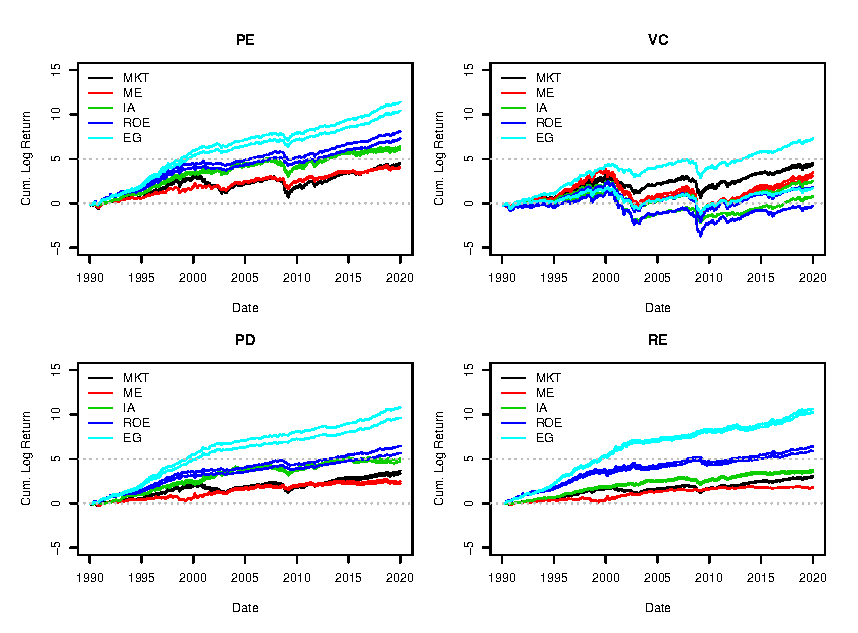
\includegraphics{eps/0_SDF_realizations_EW}
	\caption{Cumulative log returns for the models displayed in tables \ref{tab:ai_40_ew_dep} and  \ref{tab:ai_60_ew_dep} that are estimated with equal-weighted cash flows.
	For each $q$-factor SDF realization there are two lines for maximum quarter 40 and 60, respectively.	
}
	\label{fig:NPV_historgram}
\end{figure}

\section{Conclusion}
\label{sec:conclusion}

Equipped with a case specific (economic) distance measure, our least-mean-distance estimator can be easily generalized to estimate SDF models for all kinds of non-traded cash flows.

As we are already in a spatial framework, we could refine the distance measure to multiple dimensions by, e.g., incorporating geographic and industry sector proximity.

We advice to always challenge asymptotic inference results in the data-sparse private equity domain by bootstrapping or cross-validation analyses that are adapted to the dependency structure of overlapping fund cash flows.


%% References
\bibliographystyle{apalike}
\bibliography{xfundwise_sdf}



% Appendix



\newpage


% Fundwise, $D=12$

% latex table generated in R 3.4.2 by xtable 1.8-4 package
% Wed Apr  8 11:36:03 2020
\begin{table}[ht]
	\centering
	\begin{tabular}{lrrlrrr}
		Type & MKT & SE.MKT & Factor & Coef & SE.Coef & Wald.p.value.MKT\_1 \\ 
		\hline
		\hline
		PE & 2.76 & 1.33 & MKT &  &  & 0.02 \\ 
		PE & 1.63 & 3.02 & ME & 1.49 & 3.17 & 0.00 \\ 
		PE & 2.34 & 1.08 & IA & 2.64 & 7.27 & 0.00 \\ 
		PE & 2.08 & 2.25 & ROE & 2.22 & 3.57 & 0.00 \\ 
		PE & 2.16 & 2.07 & EG & 2.83 & 6.61 & 0.00 \\
		\hline
		VC & 2.87 & 1.45 & MKT &  &  & 0.01 \\ 
		VC & 3.71 & 5.72 & ME & -1.78 & 6.43 & 0.00 \\ 
		VC & 2.79 & 1.40 & IA & -1.65 & 4.14 & 0.00 \\ 
		VC & 3.09 & 1.69 & ROE & -1.09 & 3.57 & 0.00 \\ 
		VC & 2.82 & 1.38 & EG & 0.95 & 5.50 & 0.00 \\ 
		\hline
		PD & 1.60 & 5.22 & MKT &  &  & 0.00 \\ 
		PD & 0.46 & 14.43 & ME & 1.68 & 5.94 & 0.00 \\ 
		PD & 1.17 & 6.95 & IA & 3.18 & 10.60 & 0.00 \\ 
		PD & 1.26 & 4.71 & ROE & 1.98 & 8.58 & 0.00 \\ 
		PD & 1.20 & 7.89 & EG & 3.24 & 3.20 & 0.00 \\ 
		\hline
		RE & 1.19 & 2.87 & MKT &  &  & 0.59 \\ 
		RE & 0.13 & 7.29 & ME & 1.35 & 4.78 & 0.00 \\ 
		RE & 0.95 & 2.32 & IA & 1.42 & 7.35 & 0.00 \\ 
		RE & 0.76 & 3.13 & ROE & 2.75 & 3.57 & 0.00 \\ 
		RE & 0.69 & 3.49 & EG & 3.69 & 6.54 & 0.00 \\ 
		\hline
		NATRES & 1.90 & 1.73 & MKT &  &  & 0.12 \\ 
		NATRES & 0.84 & 1.49 & ME & 1.68 & 1.79 & 0.01 \\ 
		NATRES & 1.64 & 1.52 & IA & 1.91 & 16.04 & 0.00 \\ 
		NATRES & 1.56 & 1.15 & ROE & 2.18 & 4.29 & 0.00 \\ 
		NATRES & 1.52 & 1.64 & EG & 2.28 & 18.23 & 0.00 \\ 
		\hline
		INF & 1.72 & 2.46 & MKT &  &  & 0.08 \\ 
		INF & 0.75 & 11.62 & ME & 1.27 & 3.52 & 0.00 \\ 
		INF & 1.73 & 3.79 & IA & -0.02 & 11.57 & 0.01 \\ 
		INF & 1.08 & 8.99 & ROE & 4.65 & 23.92 & 0.00 \\ 
		INF & 1.09 & 7.84 & EG & 3.97 & 4.13 & 0.00 \\ 
		\hline
	\end{tabular}
	\caption{Asymptotic inference with equal-weighting, max quarter 40, and $D=12$. The Wald test null hypothesis is a MKT coefficient of one, and zeros for all other coefficients.} 
		\label{tab:ai_40_ew_dep} 
\end{table}


% latex table generated in R 3.4.2 by xtable 1.8-4 package
% Wed Apr  8 11:37:43 2020
\begin{table}[ht]
	\centering
	\begin{tabular}{lrrlrrl}
		Type & MKT & SE.MKT & Factor & Coef & SE.Coef & validation.error \\ 
		\hline
		\hline
		INF & 2.00 & 0.73 & MKT &  &  & 3186* \\ 
		INF & 1.27 & 1.14 & ME & 1.03 & 0.74 & 3333 \\ 
		INF & 2.01 & 0.65 & IA & -0.55 & 1.26 & 3221 \\ 
		INF & 1.36 & 0.68 & ROE & 4.57 & 2.07 & 3043 \\ 
		INF & 1.52 & 0.91 & EG & 3.78 & 0.78 & 4307 \\ 
		\hline
		NATRES & 2.03 & 0.42 & MKT &  &  & 7340 \\ 
		NATRES & 1.01 & 0.80 & ME & 1.80 & 0.63 & 9146 \\ 
		NATRES & 1.83 & 0.49 & IA & 1.79 & 0.87 & 7670 \\ 
		NATRES & 1.61 & 0.52 & ROE & 2.49 & 1.37 & 8183 \\ 
		NATRES & 1.67 & 0.47 & EG & 2.26 & 0.40 & 6933* \\ 
		\hline
		PD & 1.50 & 0.46 & MKT &  &  & 3098 \\ 
		PD & 0.50 & 0.29 & ME & 1.67 & 0.15 & 2998 \\ 
		PD & 1.15 & 0.33 & IA & 3.13 & 0.52 & 2896 \\ 
		PD & 1.16 & 0.53 & ROE & 2.05 & 0.36 & 2756* \\ 
		PD & 1.13 & 0.40 & EG & 3.22 & 0.48 & 2906 \\ 
		\hline
		PE & 2.79 & 0.20 & MKT &  &  & 1108 \\ 
		PE & 1.72 & 0.37 & ME & 1.57 & 0.24 & 1053 \\ 
		PE & 2.42 & 0.24 & IA & 2.71 & 0.40 & 1013* \\ 
		PE & 2.03 & 0.25 & ROE & 2.29 & 0.44 & 1297 \\ 
		PE & 2.14 & 0.19 & EG & 2.84 & 0.26 & 1039 \\ 
		\hline
		RE & 1.39 & 0.79 & MKT &  &  & 1893 \\ 
		RE & 0.38 & 0.64 & ME & 1.52 & 0.67 & 1723 \\ 
		RE & 1.18 & 0.92 & IA & 1.85 & 0.62 & 1767 \\ 
		RE & 0.77 & 0.43 & ROE & 2.94 & 1.03 & 1963 \\ 
		RE & 0.87 & 0.67 & EG & 3.48 & 0.47 & 1221* \\ 
		\hline
		VC & 2.81 & 0.58 & MKT &  &  & 926* \\ 
		VC & 3.39 & 0.76 & ME & -1.30 & 1.23 & 1110 \\ 
		VC & 2.69 & 0.57 & IA & -1.08 & 1.34 & 961 \\ 
		VC & 2.86 & 0.79 & ROE & -0.48 & 1.61 & 1126 \\ 
		VC & 2.54 & 0.84 & EG & 1.44 & 1.58 & 984 \\ 
		\hline
		\hline
	\end{tabular}
	\caption{$hv$-block cross-validation with max quarter 40 and equal-weighted cash flows.}
	\label{tab:cv_40_ew_dep} 
\end{table}


% latex table generated in R 3.4.2 by xtable 1.8-4 package
% Wed Apr  8 11:36:03 2020
\begin{table}[ht]
	\centering
	\begin{tabular}{lrrlrrr}
		Type & MKT & SE.MKT & Factor & Coef & SE.Coef & Wald.p.value.MKT\_1 \\ 
		\hline
		\hline
		PE & 2.52 & 1.81 & MKT &  &  & 0.01 \\ 
		PE & 1.59 & 3.43 & ME & 1.23 & 4.68 & 0.00 \\ 
		PE & 2.15 & 2.34 & IA & 2.45 & 7.87 & 0.00 \\ 
		PE & 1.94 & 3.56 & ROE & 1.81 & 5.17 & 0.00 \\ 
		PE & 1.99 & 3.37 & EG & 2.48 & 6.69 & 0.00 \\ 
		\hline
		VC & 2.33 & 1.00 & MKT &  &  & 0.19 \\ 
		VC & 3.48 & 5.71 & ME & -2.18 & 6.32 & 0.00 \\ 
		VC & 2.20 & 1.05 & IA & -2.82 & 4.64 & 0.00 \\ 
		VC & 2.77 & 1.55 & ROE & -1.92 & 3.49 & 0.00 \\ 
		VC & 2.40 & 1.00 & EG & -0.89 & 5.65 & 0.00 \\ 
		\hline
		PD & 1.38 & 10.19 & MKT &  &  & 0.00 \\ 
		PD & 0.36 & 28.10 & ME & 1.51 & 14.36 & 0.00 \\ 
		PD & 0.98 & 13.30 & IA & 3.18 & 13.83 & 0.00 \\ 
		PD & 1.07 & 6.03 & ROE & 1.68 & 10.56 & 0.00 \\ 
		PD & 1.02 & 9.89 & EG & 2.86 & 5.77 & 0.00 \\ 
		\hline
		RE & 1.11 & 3.07 & MKT &  &  & 0.74 \\ 
		RE & 0.16 & $0.02^{!!!}$ & ME & 1.19 & $0.03^{!!!}$ & $1.00^{!!!}$ \\ 
		RE & 0.89 & 2.52 & IA & 1.31 & 7.36 & 0.00 \\ 
		RE & 0.67 & 3.27 & ROE & 2.50 & 5.06 & 0.00 \\ 
		RE & 0.62 & 4.35 & EG & 3.57 & 7.32 & 0.00 \\ 
		\hline
		NATRES & 1.61 & 1.23 & MKT &  &  & 0.45 \\ 
		NATRES & 0.88 & 5.09 & ME & 1.17 & 7.58 & 0.00 \\ 
		NATRES & 1.36 & 1.28 & IA & 1.96 & 15.53 & 0.00 \\ 
		NATRES & 1.34 & 1.36 & ROE & 1.74 & 6.94 & 0.00 \\ 
		NATRES & 1.27 & 1.54 & EG & 2.18 & 17.57 & 0.00 \\ 
		\hline
		INF & 1.65 & 2.44 & MKT &  &  & 0.11 \\ 
		INF & 0.65 & 11.78 & ME & 1.32 & 3.48 & 0.00 \\ 
		INF & 1.62 & 2.09 & IA & 0.21 & 5.14 & 0.18 \\ 
		INF & 1.07 & 8.98 & ROE & 4.67 & 23.97 & 0.00 \\ 
		INF & 1.09 & 7.85 & EG & 3.91 & 4.20 & 0.00 \\ 
		\hline
		\hline
	\end{tabular}
	\caption{
		Asymptotic inference with max quarter 60 and equal-weighted cash flows.
		Numerical issues within the asymptotic covariance matrix estimation seem to cause the dubious values with superscript $x^{!!!}$; the corresponding estimates for columns MKT and Coef are not affected and stay valid.
	}
	\label{tab:ai_60_ew_dep} 
\end{table}


% latex table generated in R 3.4.2 by xtable 1.8-4 package
% Wed Apr  8 11:37:43 2020
\begin{table}[ht]
	\centering
	\begin{tabular}{lrrlrrl}
		Type & MKT & SE.MKT & Factor & Coef & SE.Coef & validation.error \\ 
		\hline
		\hline
		INF & 1.95 & 0.76 & MKT &  &  & 3234* \\ 
		INF & 1.18 & 1.20 & ME & 1.08 & 0.76 & 3400 \\ 
		INF & 1.90 & 0.75 & IA & -0.21 & 1.24 & 3265 \\ 
		INF & 1.38 & 0.69 & ROE & 4.50 & 2.20 & 3494 \\ 
		INF & 1.56 & 1.00 & EG & 3.67 & 0.88 & 4872 \\ 
		\hline
		NATRES & 1.70 & 0.37 & MKT &  &  & 8055 \\ 
		NATRES & 0.90 & 0.83 & ME & 1.31 & 0.56 & 10577 \\ 
		NATRES & 1.50 & 0.46 & IA & 1.82 & 0.91 & 8414 \\ 
		NATRES & 1.36 & 0.44 & ROE & 2.05 & 1.36 & 9469 \\ 
		NATRES & 1.38 & 0.40 & EG & 2.15 & 0.39 & 7782* \\ 
		\hline
		PD & 1.24 & 0.58 & MKT &  &  & 3334 \\ 
		PD & 0.32 & 0.34 & ME & 1.49 & 0.19 & 3403 \\ 
		PD & 0.91 & 0.45 & IA & 3.05 & 0.43 & 3276 \\ 
		PD & 0.94 & 0.60 & ROE & 1.72 & 0.32 & 3173* \\ 
		PD & 0.92 & 0.50 & EG & 2.82 & 0.45 & 3458 \\ 
		\hline
		PE & 2.52 & 0.25 & MKT &  &  & 1199 \\ 
		PE & 1.61 & 0.32 & ME & 1.29 & 0.24 & 1217 \\ 
		PE & 2.17 & 0.21 & IA & 2.52 & 0.40 & 1132* \\ 
		PE & 1.87 & 0.29 & ROE & 1.86 & 0.34 & 1380 \\ 
		PE & 1.96 & 0.24 & EG & 2.51 & 0.24 & 1155 \\ 
		\hline
		RE & 1.27 & 0.79 & MKT &  &  & 1993 \\ 
		RE & 0.37 & 0.58 & ME & 1.33 & 0.59 & 1871 \\ 
		RE & 1.07 & 0.89 & IA & 1.70 & 0.60 & 1879 \\ 
		RE & 0.68 & 0.45 & ROE & 2.70 & 0.96 & 1953 \\ 
		RE & 0.78 & 0.66 & EG & 3.36 & 0.46 & 1262* \\
		\hline
		VC & 2.29 & 0.69 & MKT &  &  & 1017* \\ 
		VC & 3.10 & 0.79 & ME & -1.70 & 1.24 & 1206 \\ 
		VC & 2.11 & 0.67 & IA & -1.95 & 2.12 & 1101 \\ 
		VC & 2.56 & 0.82 & ROE & -1.27 & 1.55 & 1275 \\ 
		VC & 2.14 & 0.90 & EG & -0.15 & 1.98 & 1165 \\ 
		\hline
		\hline
	\end{tabular}
	\caption{$hv$-block cross-validation with equal-weighting, max quarter 60, and $D=12$. The Wald test null hypothesis is a MKT coefficient of one, and zeros for all other coefficients.}
	\label{tab:cv_60_ew_dep} 
\end{table}



% latex table generated in R 3.4.2 by xtable 1.8-4 package
% Wed Apr  8 21:59:13 2020
\begin{table}[ht]
	\centering
	\begin{tabular}{lrrlrrr}
		Type & MKT & SE.MKT & Factor & Coef & SE.Coef & Wald.p.value.MKT\_1 \\ 
		\hline
		\hline
		PE & 2.67 & 1.77 & MKT &  &  & 0.00 \\ 
		PE & 1.39 & 8.25 & ME & 1.36 & 3.37 & 0.00 \\ 
		PE & 1.97 & 2.54 & IA & 3.36 & 14.56 & 0.00 \\ 
		PE & 2.20 & 2.26 & ROE & 3.15 & 3.48 & 0.00 \\ 
		PE & 1.94 & 3.98 & EG & 3.83 & 5.89 & 0.00 \\ 
		\hline
		VC & 2.46 & 1.86 & MKT &  &  & 0.01 \\ 
		VC & 3.30 & 7.04 & ME & -1.13 & 8.55 & 0.00 \\ 
		VC & 2.48 & 1.92 & IA & -0.52 & 5.81 & 0.00 \\ 
		VC & 2.48 & 1.85 & ROE & -0.10 & 4.12 & 0.02 \\ 
		VC & 2.37 & 1.56 & EG & 0.67 & 9.13 & 0.00 \\ 
		\hline
		PD & 1.73 & 487.52 & MKT &  &  & 0.00 \\ 
		PD & 1.33 & 70.41 & ME & 0.57 & 53.48 & 0.00 \\ 
		PD & 1.64 & 33.58 & IA & 0.73 & 17.61 & 0.00 \\ 
		PD & 2.01 & 114.44 & ROE & 2.57 & 159.48 & 0.00 \\ 
		PD & 1.43 & 2.18 & EG & 3.96 & 20.34 & 0.00 \\ 
		\hline
		RE & 1.33 & 1.87 & MKT &  &  & 0.54 \\ 
		RE & -0.36 & 8.88 & ME & 2.07 & 7.69 & 0.00 \\ 
		RE & 1.12 & 2.10 & IA & 1.24 & 5.34 & 0.00 \\ 
		RE & 1.14 & 2.11 & ROE & 3.68 & 2.68 & 0.00 \\ 
		RE & 0.58 & 3.63 & EG & 6.60 & 6.63 & 0.00 \\ 
		\hline
		NATRES & -0.19 & 1.28 & MKT &  &  & 0.13 \\ 
		NATRES & -1.56 & 16.46 & ME & 1.66 & 20.46 & 0.00 \\ 
		NATRES & -0.95 & 2.91 & IA & 3.40 & 4.31 & 0.00 \\ 
		NATRES & -0.31 & 1.90 & ROE & 3.37 & 3.19 & 0.00 \\ 
		NATRES & -0.73 & 2.68 & EG & 4.72 & 3.05 & 0.00 \\ 
		\hline
		INF & 2.42 & 3.61 & MKT &  &  & 0.00 \\ 
		INF & 3.96 & 63.33 & ME & -2.33 & 90.63 & 0.00 \\ 
		INF & 1.72 & 1.24 & IA & 3.44 & 2.75 & 0.00 \\ 
		INF & 1.31 & 8.31 & ROE & 6.08 & 62.75 & 0.00 \\ 
		INF & 1.64 & 1.53 & EG & 5.96 & 4.80 & 0.00 \\ 
		\hline
		\hline
	\end{tabular}
	\caption{Asymptotic inference with fund-size-weighting, max quarter 40, and $D=12$. The Wald test null hypothesis is a MKT coefficient of one, and zeros for all other coefficients.}
	\label{tab:ai_40_fw_dep}
\end{table}


% latex table generated in R 3.4.2 by xtable 1.8-4 package
% Wed Apr  8 21:59:13 2020
\begin{table}[ht]
	\centering
	\begin{tabular}{lrrlrrl}
		Type & MKT & SE.MKT & Factor & Coef & SE.Coef & validation.error \\ 
		\hline
		\hline
		INF & 3.19 & 1.96 & MKT &  &  & 3762 \\ 
		INF & 3.81 & 2.34 & ME & -1.42 & 1.32 & 3160 \\ 
		INF & 2.42 & 1.32 & IA & 4.16 & 4.75 & 4332 \\ 
		INF & 1.56 & 0.81 & ROE & 5.65 & 1.10 & 1684* \\ 
		INF & 2.67 & 1.93 & EG & 5.79 & 1.69 & 4603 \\ 
		\hline
		NATRES & 0.19 & 0.75 & MKT &  &  & 2792 \\ 
		NATRES & -1.08 & 1.05 & ME & 1.61 & 0.68 & 3056 \\ 
		NATRES & -0.44 & 0.92 & IA & 3.76 & 0.78 & 2830 \\ 
		NATRES & -0.09 & 0.53 & ROE & 3.36 & 0.49 & 2866 \\ 
		NATRES & -0.35 & 0.83 & EG & 4.56 & 1.07 & 2738* \\ 
		\hline
		PD & 1.64 & 0.40 & MKT &  &  & 1081 \\ 
		PD & 1.38 & 0.56 & ME & 0.62 & 0.91 & 1132 \\ 
		PD & 1.60 & 0.32 & IA & 1.44 & 1.94 & 1080 \\ 
		PD & 1.79 & 0.46 & ROE & 2.61 & 0.21 & 991 \\ 
		PD & 1.41 & 0.19 & EG & 3.87 & 0.21 & 834* \\ 
		\hline
		PE & 3.03 & 0.71 & MKT &  &  & 923* \\ 
		PE & 1.99 & 0.84 & ME & 1.42 & 0.62 & 1018 \\ 
		PE & 2.44 & 0.79 & IA & 3.45 & 1.43 & 944 \\ 
		PE & 2.29 & 0.25 & ROE & 3.12 & 0.52 & 1253 \\ 
		PE & 2.29 & 0.64 & EG & 3.61 & 0.44 & 1033 \\ 
		\hline
		RE & 1.79 & 1.34 & MKT &  &  & 2599 \\ 
		RE & 0.17 & 1.52 & ME & 2.16 & 0.66 & 2558* \\ 
		RE & 1.33 & 1.70 & IA & 2.53 & 2.47 & 2619 \\ 
		RE & 1.39 & 0.96 & ROE & 3.69 & 1.41 & 4163 \\ 
		RE & 1.10 & 1.43 & EG & 5.56 & 2.70 & 3836 \\ 
		\hline
		VC & 2.52 & 0.48 & MKT &  &  & 581* \\ 
		VC & 2.88 & 1.25 & ME & -0.63 & 1.29 & 719 \\ 
		VC & 2.41 & 0.57 & IA & -0.11 & 1.60 & 627 \\ 
		VC & 2.42 & 0.75 & ROE & 0.34 & 1.57 & 700 \\ 
		VC & 2.27 & 0.75 & EG & 1.12 & 1.79 & 633 \\ 
		\hline
		\hline
	\end{tabular}
	\caption{$hv$-block cross-validation with max quarter 40 and fund-size-weighting.}
	\label{tab:cv_40_fw_dep}
\end{table}


% latex table generated in R 3.4.2 by xtable 1.8-4 package
% Wed Apr  8 21:59:13 2020
\begin{table}[ht]
	\centering
	\begin{tabular}{lrrlrrr}
		Type & MKT & SE.MKT & Factor & Coef & SE.Coef & Wald.p.value.MKT\_1 \\ 
		\hline
		\hline
		PE & 2.55 & 1.82 & MKT &  &  & 0.00 \\ 
		PE & 1.28 & 11.10 & ME & 1.32 & 2.73 & 0.00 \\ 
		PE & 1.92 & 4.04 & IA & 2.90 & 15.64 & 0.00 \\ 
		PE & 2.11 & 3.82 & ROE & 2.63 & 4.89 & 0.00 \\ 
		PE & 1.90 & 5.33 & EG & 3.30 & 8.52 & 0.00 \\ 
		\hline
		VC & 2.16 & 1.46 & MKT &  &  & 0.09 \\ 
		VC & 3.25 & 7.13 & ME & -1.37 & 8.69 & 0.00 \\ 
		VC & 2.21 & 1.55 & IA & -1.24 & 6.94 & 0.00 \\ 
		VC & 2.33 & 1.54 & ROE & -0.78 & 4.44 & 0.00 \\ 
		VC & 2.24 & 1.52 & EG & -0.52 & 8.67 & 0.00 \\ 
		\hline
		PD & 1.69 & 278.63 & MKT &  &  & 0.00 \\ 
		PD & 1.30 & 46.16 & ME & 0.55 & 50.65 & 0.00 \\ 
		PD & 1.52 & 32.87 & IA & 1.25 & 17.26 & 0.00 \\ 
		PD & 1.92 & 16.68 & ROE & 2.38 & 25.01 & 0.00 \\ 
		PD & 1.40 & 2.23 & EG & 3.95 & 20.71 & 0.00 \\ 
		\hline
		RE & 1.27 & 2.25 & MKT &  &  & 0.54 \\ 
		RE & -0.27 & 8.46 & ME & 1.88 & 6.93 & 0.00 \\ 
		RE & 1.07 & 2.15 & IA & 1.21 & 5.27 & 0.00 \\ 
		RE & 1.04 & 2.17 & ROE & 3.23 & 3.28 & 0.00 \\ 
		RE & 0.54 & 3.56 & EG & 6.04 & 4.42 & 0.00 \\ 
		\hline
		NATRES & -0.26 & 1.34 & MKT &  &  & 0.09 \\ 
		NATRES & -1.49 & 16.31 & ME & 1.51 & 19.98 & 0.00 \\ 
		NATRES & -1.00 & 3.57 & IA & 3.29 & 7.08 & 0.00 \\ 
		NATRES & -0.37 & 1.99 & ROE & 3.16 & 3.30 & 0.00 \\ 
		NATRES & -0.77 & 2.68 & EG & 4.55 & 3.09 & 0.00 \\ 
		\hline
		INF & 2.34 & 3.65 & MKT &  &  & 0.00 \\ 
		INF & 3.85 & 65.89 & ME & -2.30 & 70.34 & 0.00 \\ 
		INF & 1.59 & 1.31 & IA & 3.81 & 2.46 & 0.00 \\ 
		INF & 1.22 & 12.07 & ROE & 6.13 & 17.26 & 0.00 \\ 
		INF & 1.63 & 1.52 & EG & 5.79 & 4.83 & 0.00 \\ 
		\hline
		\hline
	\end{tabular}
	\caption{Asymptotic inference with fund-size-weighting, max quarter 60, and $D=12$. The Wald test null hypothesis is a MKT coefficient of one, and zeros for all other coefficients.}
	\label{tab:ai_60_fw_dep}
\end{table}



% latex table generated in R 3.4.2 by xtable 1.8-4 package
% Wed Apr  8 21:59:13 2020
\begin{table}[ht]
	\centering
	\begin{tabular}{lrrlrrl}
		Type & MKT & SE.MKT & Factor & Coef & SE.Coef & validation.error \\ 
		\hline
		\hline
		INF & 3.15 & 2.00 & MKT &  &  & 3913 \\ 
		INF & 3.69 & 2.46 & ME & -1.33 & 1.45 & 3301 \\ 
		INF & 2.25 & 1.47 & IA & 4.78 & 3.86 & 4429 \\ 
		INF & 1.54 & 0.83 & ROE & 5.67 & 1.03 & 1961* \\ 
		INF & 2.65 & 1.98 & EG & 5.86 & 1.54 & 5111 \\ 
		\hline
		NATRES & 0.04 & 0.65 & MKT &  &  & 2771 \\ 
		NATRES & -1.12 & 0.97 & ME & 1.47 & 0.64 & 3037 \\ 
		NATRES & -0.59 & 0.79 & IA & 3.60 & 0.71 & 2725* \\ 
		NATRES & -0.22 & 0.43 & ROE & 3.15 & 0.50 & 3140 \\ 
		NATRES & -0.46 & 0.73 & EG & 4.39 & 1.02 & 2772 \\ 
		\hline
		PD & 1.57 & 0.46 & MKT &  &  & 1154 \\ 
		PD & 1.35 & 0.63 & ME & 0.54 & 0.90 & 1205 \\ 
		PD & 1.47 & 0.35 & IA & 1.82 & 1.63 & 1101 \\ 
		PD & 1.69 & 0.49 & ROE & 2.43 & 0.25 & 1173 \\ 
		PD & 1.34 & 0.25 & EG & 3.76 & 0.38 & 979* \\ 
		\hline
		PE & 2.74 & 0.50 & MKT &  &  & 970 \\ 
		PE & 1.74 & 0.67 & ME & 1.31 & 0.55 & 1046 \\ 
		PE & 2.19 & 0.50 & IA & 2.84 & 1.43 & 964* \\ 
		PE & 2.11 & 0.20 & ROE & 2.60 & 0.37 & 1426 \\ 
		PE & 2.09 & 0.44 & EG & 3.12 & 0.48 & 1127 \\ 
		\hline
		RE & 1.63 & 1.35 & MKT &  &  & 2759* \\ 
		RE & 0.16 & 1.45 & ME & 1.89 & 0.72 & 2771 \\ 
		RE & 1.15 & 1.71 & IA & 2.52 & 2.64 & 2803 \\ 
		RE & 1.25 & 1.06 & ROE & 3.29 & 1.34 & 4445 \\ 
		RE & 0.95 & 1.42 & EG & 5.11 & 2.60 & 4063 \\ 
		\hline
		VC & 2.20 & 0.43 & MKT &  &  & 626* \\ 
		VC & 2.80 & 1.12 & ME & -0.90 & 1.25 & 779 \\ 
		VC & 2.09 & 0.50 & IA & -0.88 & 2.10 & 692 \\ 
		VC & 2.23 & 0.67 & ROE & -0.33 & 1.50 & 781 \\ 
		VC & 2.09 & 0.68 & EG & -0.02 & 2.06 & 718 \\ 
		\hline
		\hline
	\end{tabular}
	\caption{$hv$-block cross-validation with max quarter 60 and fund-size-weighting.}
	\label{tab:cv_60_fw_dep}
\end{table}



% Fundwise, $D<1$



% latex table generated in R 3.4.2 by xtable 1.8-4 package
% Fri Apr 10 10:55:27 2020
\begin{table}[ht]
	\centering
	\begin{tabular}{lrrlrrr}
		Type & MKT & SE.MKT & Factor & Coef & SE.Coef & Wald.p.value.MKT\_1 \\ 
		\hline
		\hline
		PE & 2.76 & 0.46 & MKT &  &  & 0.41 \\ 
		PE & 1.63 & 0.47 & ME & 1.49 & 0.47 & 0.84 \\ 
		PE & 2.34 & 0.39 & IA & 2.64 & 0.89 & 0.07 \\ 
		PE & 2.08 & 0.58 & ROE & 2.22 & 0.53 & 0.63 \\ 
		PE & 2.16 & 0.50 & EG & 2.83 & 1.03 & 0.02 \\ 
		\hline
		VC & 2.87 & 0.51 & MKT &  &  & 0.34 \\ 
		VC & 3.71 & 0.73 & ME & -1.78 & 0.63 & 0.02 \\ 
		VC & 2.79 & 0.56 & IA & -1.65 & 1.19 & 0.08 \\ 
		VC & 3.09 & 0.52 & ROE & -1.09 & 0.67 & 0.46 \\ 
		VC & 2.82 & 0.48 & EG & 0.95 & 1.24 & 0.38 \\ 
		\hline
		PD & 1.60 & 2.12 & MKT &  &  & 0.21 \\ 
		PD & 0.46 & 2.65 & ME & 1.68 & 2.29 & 0.00 \\ 
		PD & 1.17 & 1.75 & IA & 3.18 & 3.58 & 0.00 \\ 
		PD & 1.26 & 3.20 & ROE & 1.98 & 3.66 & 0.00 \\ 
		PD & 1.20 & 2.70 & EG & 3.24 & 5.63 & 0.00 \\ 
		\hline
		RE & 1.19 & 0.94 & MKT &  &  & 0.86 \\ 
		RE & 0.13 & 1.20 & ME & 1.35 & 1.23 & 0.04 \\ 
		RE & 0.95 & 0.84 & IA & 1.42 & 2.15 & 0.01 \\ 
		RE & 0.76 & 1.08 & ROE & 2.75 & 0.83 & 0.05 \\ 
		RE & 0.69 & 0.96 & EG & 3.69 & 3.35 & 0.00 \\ 
		\hline
		NATRES & 1.90 & 1.33 & MKT &  &  & 0.23 \\ 
		NATRES & 0.84 & 2.47 & ME & 1.68 & 3.40 & 0.00 \\ 
		NATRES & 1.64 & 1.74 & IA & 1.91 & 11.79 & 0.00 \\ 
		NATRES & 1.56 & 1.44 & ROE & 2.18 & 3.18 & 0.00 \\ 
		NATRES & 1.52 & 1.86 & EG & 2.28 & 15.15 & 0.00 \\ 
		\hline
		INF & 1.72 & 5.43 & MKT &  &  & 0.00 \\ 
		INF & 0.75 & 4.36 & ME & 1.27 & 2.89 & 0.00 \\ 
		INF & 1.73 & 7.55 & IA & -0.02 & 11.12 & 0.00 \\ 
		INF & 1.08 & 3.64 & ROE & 4.65 & 16.93 & 0.00 \\ 
		INF & 1.09 & 3.58 & EG & 3.97 & 9.01 & 0.00 \\ 
		\hline
		\hline
	\end{tabular}
	\caption{Asymptotic inference with equal-weighting, max quarter 40, and $D<1$.. The Wald test null hypothesis is a MKT coefficient of one, and zeros for all other coefficients.}
	\label{tab:ai_40_ew_indep}
\end{table}

% latex table generated in R 3.4.2 by xtable 1.8-4 package
% Fri Apr 10 10:55:27 2020
\begin{table}[ht]
	\centering
	\begin{tabular}{lrrlrrr}
		Type & MKT & SE.MKT & Factor & Coef & SE.Coef & Wald.p.value.MKT\_1 \\ 
		\hline
		\hline
		PE & 2.52 & 0.53 & MKT &  &  & 0.42 \\ 
		PE & 1.59 & 0.52 & ME & 1.23 & 0.51 & 0.85 \\ 
		PE & 2.15 & 0.45 & IA & 2.45 & 0.95 & 0.07 \\ 
		PE & 1.94 & 0.67 & ROE & 1.81 & 0.67 & 0.58 \\ 
		PE & 1.99 & 0.55 & EG & 2.48 & 1.04 & 0.05 \\ 
		\hline
		VC & 2.33 & 0.55 & MKT &  &  & 0.46 \\ 
		VC & 3.48 & 0.73 & ME & -2.18 & 0.58 & 0.02 \\ 
		VC & 2.20 & 0.55 & IA & -2.82 & 1.03 & 0.01 \\ 
		VC & 2.77 & 0.46 & ROE & -1.92 & 0.66 & 0.28 \\ 
		VC & 2.40 & 0.55 & EG & -0.89 & 0.99 & 0.50 \\ 
		\hline
		PD & 1.38 & 2.95 & MKT &  &  & 0.26 \\ 
		PD & 0.36 & 5.60 & ME & 1.51 & 5.05 & 0.00 \\ 
		PD & 0.98 & 2.90 & IA & 3.18 & 3.91 & 0.00 \\ 
		PD & 1.07 & 3.68 & ROE & 1.68 & 4.32 & 0.00 \\ 
		PD & 1.02 & 2.88 & EG & 2.86 & 5.56 & 0.00 \\ 
		\hline
		RE & 1.11 & 0.97 & MKT &  &  & 0.92 \\ 
		RE & 0.16 & 0.01 & ME & 1.19 & 0.01 & 1.00 \\ 
		RE & 0.89 & 0.87 & IA & 1.31 & 2.14 & 0.02 \\ 
		RE & 0.67 & 1.23 & ROE & 2.50 & 1.19 & 0.01 \\ 
		RE & 0.62 & 1.00 & EG & 3.57 & 3.39 & 0.00 \\ 
		\hline
		NATRES & 1.61 & 1.33 & MKT &  &  & 0.41 \\ 
		NATRES & 0.88 & 3.54 & ME & 1.17 & 4.66 & 0.00 \\ 
		NATRES & 1.36 & 1.73 & IA & 1.96 & 11.42 & 0.00 \\ 
		NATRES & 1.34 & 1.41 & ROE & 1.74 & 3.99 & 0.00 \\ 
		NATRES & 1.27 & 1.88 & EG & 2.18 & 14.70 & 0.00 \\ 
		\hline
		INF & 1.65 & 5.34 & MKT &  &  & 0.00 \\ 
		INF & 0.65 & 4.33 & ME & 1.32 & 2.88 & 0.00 \\ 
		INF & 1.62 & 4.90 & IA & 0.21 & 4.41 & 0.01 \\ 
		INF & 1.07 & 3.63 & ROE & 4.67 & 16.96 & 0.00 \\ 
		INF & 1.09 & 3.57 & EG & 3.91 & 9.17 & 0.00 \\ 
		\hline
		\hline
	\end{tabular}
	\caption{Asymptotic inference with equal-weighting, max quarter 60, and $D<1$. The Wald test null hypothesis is a MKT coefficient of one, and zeros for all other coefficients.}
	\label{tab:ai_60_ew_indep}
\end{table}


% latex table generated in R 3.4.2 by xtable 1.8-4 package
% Fri Apr 10 10:47:44 2020
\begin{table}[ht]
	\centering
	\begin{tabular}{lrrlrrr}
		Type & MKT & SE.MKT & Factor & Coef & SE.Coef & Wald.p.value.MKT\_1 \\ 
		\hline
		\hline
		PE & 2.67 & 1.21 & MKT &  &  & 0.04 \\ 
		PE & 1.39 & 1.45 & ME & 1.36 & 1.30 & 0.31 \\ 
		PE & 1.97 & 1.03 & IA & 3.36 & 2.12 & 0.00 \\ 
		PE & 2.20 & 1.48 & ROE & 3.15 & 0.86 & 0.17 \\ 
		PE & 1.94 & 1.30 & EG & 3.83 & 1.64 & 0.00 \\ 
		\hline
		VC & 2.46 & 0.79 & MKT &  &  & 0.25 \\ 
		VC & 3.30 & 1.14 & ME & -1.13 & 1.06 & 0.00 \\ 
		VC & 2.48 & 0.84 & IA & -0.52 & 1.53 & 0.42 \\ 
		VC & 2.48 & 0.78 & ROE & -0.10 & 0.82 & 0.52 \\ 
		VC & 2.37 & 0.80 & EG & 0.67 & 1.73 & 0.20 \\ 
		\hline
		PD & 1.73 & 463.99 & MKT &  &  & 0.00 \\ 
		PD & 1.33 & 114.73 & ME & 0.57 & 74.73 & 0.00 \\ 
		PD & 1.64 & 15.65 & IA & 0.73 & 17.37 & 0.00 \\ 
		PD & 2.01 & 40.83 & ROE & 2.57 & 59.09 & 0.00 \\ 
		PD & 1.43 & 5.01 & EG & 3.96 & 12.80 & 0.00 \\ 
		\hline
		RE & 1.33 & 1.04 & MKT &  &  & 0.73 \\ 
		RE & -0.36 & 1.75 & ME & 2.07 & 1.77 & 0.00 \\ 
		RE & 1.12 & 1.46 & IA & 1.24 & 3.69 & 0.00 \\ 
		RE & 1.14 & 1.70 & ROE & 3.68 & 1.00 & 0.00 \\ 
		RE & 0.58 & 1.54 & EG & 6.60 & 3.74 & 0.00 \\
		\hline 
		NATRES & -0.19 & 2.28 & MKT &  &  & 0.01 \\ 
		NATRES & -1.56 & 6.03 & ME & 1.66 & 8.34 & 0.00 \\ 
		NATRES & -0.95 & 2.06 & IA & 3.40 & 3.67 & 0.00 \\ 
		NATRES & -0.31 & 2.39 & ROE & 3.37 & 2.87 & 0.00 \\ 
		NATRES & -0.73 & 2.17 & EG & 4.72 & 2.34 & 0.00 \\ 
		\hline
		INF & 2.42 & 2.55 & MKT &  &  & 0.00 \\ 
		INF & 3.96 & 22.11 & ME & -2.33 & 31.17 & 0.00 \\ 
		INF & 1.72 & 2.10 & IA & 3.44 & 3.82 & 0.00 \\ 
		INF & 1.31 & 16.86 & ROE & 6.08 & 78.81 & 0.00 \\ 
		INF & 1.64 & 2.15 & EG & 5.96 & 5.70 & 0.00 \\ 
		\hline
		\hline
	\end{tabular}
	\caption{Asymptotic inference with fund-size-weighting, max quarter 40, and $D<1$. The Wald test null hypothesis is a MKT coefficient of one, and zeros for all other coefficients.}
	\label{tab:ai_40_fw_indep}
\end{table}

% latex table generated in R 3.4.2 by xtable 1.8-4 package
% Fri Apr 10 10:47:44 2020
\begin{table}[ht]
	\centering
	\begin{tabular}{lrrlrrr}
		Type & MKT & SE.MKT & Factor & Coef & SE.Coef & Wald.p.value.MKT\_1 \\ 
		\hline
		\hline
		PE & 2.55 & 1.32 & MKT &  &  & 0.04 \\ 
		PE & 1.28 & 1.63 & ME & 1.32 & 1.31 & 0.30 \\ 
		PE & 1.92 & 1.25 & IA & 2.90 & 2.17 & 0.00 \\ 
		PE & 2.11 & 1.66 & ROE & 2.63 & 1.08 & 0.11 \\ 
		PE & 1.90 & 1.49 & EG & 3.30 & 2.05 & 0.00 \\ 
		\hline
		VC & 2.16 & 0.83 & MKT &  &  & 0.34 \\ 
		VC & 3.25 & 1.16 & ME & -1.37 & 1.03 & 0.00 \\ 
		VC & 2.21 & 0.82 & IA & -1.24 & 1.40 & 0.14 \\ 
		VC & 2.33 & 0.81 & ROE & -0.78 & 0.75 & 0.51 \\ 
		VC & 2.24 & 0.82 & EG & -0.52 & 1.39 & 0.50 \\ 
		\hline
		PD & 1.69 & 255.77 & MKT &  &  & 0.00 \\ 
		PD & 1.30 & 37.95 & ME & 0.55 & 20.26 & 0.01 \\ 
		PD & 1.52 & 15.09 & IA & 1.25 & 16.89 & 0.00 \\ 
		PD & 1.92 & 6.17 & ROE & 2.38 & 12.45 & 0.00 \\ 
		PD & 1.40 & 5.00 & EG & 3.95 & 12.72 & 0.00 \\ 
		\hline
		RE & 1.27 & 1.49 & MKT &  &  & 0.68 \\ 
		RE & -0.27 & 1.50 & ME & 1.88 & 1.59 & 0.00 \\ 
		RE & 1.07 & 1.48 & IA & 1.21 & 3.65 & 0.00 \\ 
		RE & 1.04 & 1.74 & ROE & 3.23 & 1.05 & 0.00 \\ 
		RE & 0.54 & 1.59 & EG & 6.04 & 4.18 & 0.00 \\ 
		\hline
		NATRES & -0.26 & 2.26 & MKT &  &  & 0.00 \\ 
		NATRES & -1.49 & 6.04 & ME & 1.51 & 8.18 & 0.00 \\ 
		NATRES & -1.00 & 2.06 & IA & 3.29 & 5.74 & 0.00 \\ 
		NATRES & -0.37 & 2.37 & ROE & 3.16 & 2.91 & 0.00 \\ 
		NATRES & -0.77 & 2.14 & EG & 4.55 & 2.42 & 0.00 \\ 
		\hline
		INF & 2.34 & 2.61 & MKT &  &  & 0.00 \\ 
		INF & 3.85 & 24.25 & ME & -2.30 & 24.97 & 0.00 \\ 
		INF & 1.59 & 2.09 & IA & 3.81 & 3.76 & 0.00 \\ 
		INF & 1.22 & 5.59 & ROE & 6.13 & 27.69 & 0.00 \\ 
		INF & 1.63 & 2.17 & EG & 5.79 & 5.82 & 0.00 \\ 
		\hline
		\hline
	\end{tabular}
	\caption{Asymptotic inference with fund-size-weighting, max quarter 60, and $D<1$. The Wald test null hypothesis is a MKT coefficient of one, and zeros for all other coefficients.}
	\label{tab:ai_60_fw_indep}
\end{table}




% Vintage year portfolios, $D=12$


% latex table generated in R 3.4.2 by xtable 1.8-4 package
% Fri Apr 10 12:06:25 2020
\begin{table}[ht]
	\centering
	\begin{tabular}{lrrlrrr}
		Type & MKT & SE.MKT & Factor & Coef & SE.Coef & Wald.p.value.MKT\_1 \\ 
		\hline
		\hline
		PE & 2.28 & 4.40 & MKT &  &  & 0.00 \\ 
		PE & 2.11 & 1579.54 & ME & 0.23 & 1867.70 & 0.00 \\ 
		PE & 2.11 & 18.94 & IA & -1.22 & 8.49 & 0.00 \\ 
		PE & 1.05 & 32.63 & ROE & 2.48 & 21.10 & 0.00 \\ 
		PE & 1.29 & 75.16 & EG & 1.40 & 27.47 & 0.00 \\ 
		\hline
		VC & 1.98 & 9.02 & MKT &  &  & 0.00 \\ 
		VC & 2.28 & 20.45 & ME & -0.56 & 8.05 & 0.00 \\ 
		VC & 1.90 & 12.21 & IA & -0.50 & 8.79 & 0.00 \\ 
		VC & 1.93 & 14.15 & ROE & 0.16 & 13.76 & 0.00 \\ 
		VC & 1.26 & 143.33 & EG & 1.38 & 208.30 & 0.00 \\ 
		\hline
		PD & 1.97 & 5.81 & MKT &  &  & 0.00 \\ 
		PD & 0.92 & 14.10 & ME & 1.49 & 10.69 & 0.00 \\ 
		PD & 2.03 & 8.20 & IA & 1.19 & 20.40 & 0.00 \\ 
		PD & 1.26 & 14.82 & ROE & 1.82 & 34.42 & 0.00 \\ 
		PD & 1.56 & 7.11 & EG & 0.81 & 13.59 & 0.00 \\ 
		\hline
		RE & 1.71 & 28.40 & MKT &  &  & 0.00 \\ 
		RE & 2.24 & 37.80 & ME & -0.75 & 22.48 & 0.00 \\ 
		RE & 1.25 & 0.00 & IA & -2.61 & 0.00 & 1.00 \\ 
		RE & 0.46 & 11022.51 & ROE & 2.96 & 70.00 & 0.00 \\ 
		RE & 0.95 & 12.68 & EG & 1.25 & 28.41 & 0.00 \\ 
		\hline
		NATRES & 1.14 & 9.85 & MKT &  &  & 0.16 \\ 
		NATRES & 0.18 & 7.51 & ME & 1.53 & 13.44 & 0.00 \\ 
		NATRES & 1.16 & 3.65 & IA & 0.10 & 8.17 & 0.70 \\ 
		NATRES & 0.07 & 78.37 & ROE & 2.32 & 512.84 & 0.00 \\ 
		NATRES & 0.35 & 9.33 & EG & 1.17 & 12.99 & 0.00 \\ 
		\hline
		INF & 1.68 & 17.42 & MKT &  &  & 0.00 \\ 
		INF & 0.92 & 10.75 & ME & 1.11 & 32.77 & 0.00 \\ 
		INF & 1.60 & 9.97 & IA & -0.28 & 14.66 & 0.00 \\ 
		INF & 0.41 & 3.91 & ROE & 2.85 & 27.78 & 0.00 \\ 
		INF & 0.76 & 10.59 & EG & 1.23 & 13.54 & 0.00 \\ 
		\hline
		\hline
	\end{tabular}
	\caption{Asymptotic inference with equal-weighting, max quarter 40, $D=12$, and vintage year portfolios. The Wald test null hypothesis is a MKT coefficient of one, and zeros for all other coefficients.}
	\label{tab:ai_40_ew_dep_vyp}
\end{table}

% latex table generated in R 3.4.2 by xtable 1.8-4 package
% Fri Apr 10 12:06:25 2020
\begin{table}[ht]
	\centering
	\begin{tabular}{lrrlrrl}
		Type & MKT & SE.MKT & Factor & Coef & SE.Coef & validation.error \\ 
		\hline
		\hline
		INF & 1.89 & 0.44 & MKT &  &  & 14252* \\ 
		INF & 1.69 & 1.37 & ME & 0.30 & 1.43 & 14839 \\ 
		INF & 2.04 & 1.21 & IA & 2.08 & 3.61 & 27483 \\ 
		INF & 0.86 & 1.06 & ROE & 1.90 & 2.11 & 16325 \\ 
		INF & 1.13 & 0.76 & EG & 0.74 & 0.82 & 15260 \\ 
		\hline
		NATRES & 1.46 & 0.85 & MKT &  &  & 17727 \\ 
		NATRES & 0.47 & 0.97 & ME & 1.53 & 0.39 & 17588 \\ 
		NATRES & 1.43 & 1.01 & IA & 0.27 & 1.46 & 21525 \\ 
		NATRES & 0.40 & 1.02 & ROE & 2.17 & 0.78 & 16994* \\ 
		NATRES & 0.73 & 0.97 & EG & 0.97 & 0.50 & 17854 \\ 
		\hline
		PD & 1.97 & 0.13 & MKT &  &  & 14930 \\ 
		PD & 0.89 & 0.31 & ME & 1.56 & 0.35 & 12541* \\ 
		PD & 2.04 & 0.34 & IA & 1.63 & 0.68 & 16842 \\ 
		PD & 1.11 & 0.41 & ROE & 1.89 & 0.32 & 14847 \\ 
		PD & 1.54 & 0.28 & EG & 0.89 & 0.34 & 14070 \\ 
		\hline
		PE & 2.40 & 0.37 & MKT &  &  & 79174 \\ 
		PE & 2.30 & 0.64 & ME & 0.16 & 0.37 & 84220 \\ 
		PE & 2.19 & 0.35 & IA & -1.14 & 0.87 & 103256 \\ 
		PE & 1.18 & 0.39 & ROE & 2.32 & 0.67 & 61878* \\ 
		PE & 1.51 & 0.38 & EG & 1.18 & 0.46 & 68779 \\ 
		\hline
		RE & 1.74 & 0.57 & MKT &  &  & 32924 \\ 
		RE & 2.21 & 0.59 & ME & -0.69 & 0.58 & 34885 \\ 
		RE & 1.46 & 0.56 & IA & -2.15 & 1.30 & 30658 \\ 
		RE & 0.58 & 0.46 & ROE & 2.62 & 0.73 & 23821* \\ 
		RE & 1.02 & 0.61 & EG & 1.07 & 0.31 & 30380 \\ 
		\hline
		VC & 2.10 & 0.63 & MKT &  &  & 17892 \\ 
		VC & 2.82 & 1.08 & ME & -1.13 & 1.47 & 28733 \\ 
		VC & 2.01 & 0.74 & IA & -0.60 & 0.89 & 19358 \\ 
		VC & 2.01 & 0.59 & ROE & 0.23 & 0.61 & 18689 \\ 
		VC & 1.41 & 0.75 & EG & 1.29 & 0.34 & 15879* \\ 
		\hline
		\hline
	\end{tabular}
	\caption{$hv$-block cross-validation with equal-weighting, max quarter 40, and vintage year portfolios.} 
	\label{tab:cv_40_ew_dep_vyp}
\end{table}

% latex table generated in R 3.4.2 by xtable 1.8-4 package
% Fri Apr 10 12:06:25 2020
\begin{table}[ht]
	\centering
	\begin{tabular}{lrrlrrr}
		Type & MKT & SE.MKT & Factor & Coef & SE.Coef & Wald.p.value.MKT\_1 \\ 
		\hline
		\hline
		PE & 2.25 & 4.43 & MKT &  &  & 0.00 \\ 
		PE & 2.08 & 9795.75 & ME & 0.25 & 11519.20 & 0.00 \\ 
		PE & 2.07 & 19.82 & IA & -1.30 & 9.00 & 0.00 \\ 
		PE & 1.12 & 31.03 & ROE & 2.31 & 20.79 & 0.00 \\ 
		PE & 1.31 & 72.55 & EG & 1.37 & 25.92 & 0.00 \\ 
		\hline
		VC & 1.90 & 8.90 & MKT &  &  & 0.00 \\ 
		VC & 2.44 & 26.84 & ME & -0.90 & 10.48 & 0.00 \\ 
		VC & 1.76 & 4.45 & IA & -1.06 & 3.46 & 0.00 \\ 
		VC & 2.00 & 131.26 & ROE & -0.29 & 157.09 & 0.00 \\ 
		VC & 1.30 & 105.66 & EG & 1.24 & 151.22 & 0.00 \\ 
		\hline
		PD & 1.89 & 6.53 & MKT &  &  & 0.00 \\ 
		PD & 0.93 & 12.92 & ME & 1.39 & 10.29 & 0.00 \\ 
		PD & 1.94 & 7.80 & IA & 1.11 & 17.73 & 0.00 \\ 
		PD & 1.25 & 13.49 & ROE & 1.64 & 43.79 & 0.00 \\ 
		PD & 1.48 & 9.84 & EG & 0.81 & 30.35 & 0.00 \\ 
		\hline
		RE & 1.66 & 26.81 & MKT &  &  & 0.00 \\ 
		RE & 2.31 & 34.40 & ME & -0.94 & 20.54 & 0.00 \\ 
		RE & 1.26 & 23.84 & IA & -2.68 & 13.15 & 0.00 \\ 
		RE & 0.51 & 119.90 & ROE & 2.83 & 42.03 & 0.00 \\ 
		RE & 0.89 & 11.18 & EG & 1.33 & 15.93 & 0.00 \\ 
		\hline
		NATRES & 1.04 & 9.98 & MKT &  &  & 0.67 \\ 
		NATRES & 0.23 & 9.28 & ME & 1.30 & 14.81 & 0.00 \\ 
		NATRES & 1.06 & 3.73 & IA & 0.08 & 7.58 & 0.84 \\ 
		NATRES & 0.32 & 79.46 & ROE & 1.68 & 211.29 & 0.00 \\ 
		NATRES & 0.36 & 9.03 & EG & 1.05 & 12.83 & 0.00 \\ 
		\hline
		INF & 1.62 & 15.36 & MKT &  &  & 0.00 \\ 
		INF & 0.86 & 10.75 & ME & 1.13 & 32.36 & 0.00 \\ 
		INF & 1.53 & 9.27 & IA & -0.35 & 14.75 & 0.00 \\ 
		INF & 0.40 & 4.07 & ROE & 2.77 & 27.53 & 0.00 \\ 
		INF & 0.75 & 2.74 & EG & 1.21 & 15.51 & 0.00 \\ 
		\hline
		\hline
	\end{tabular}
	\caption{Asymptotic inference with equal-weighting, max quarter 60, $D=12$, and vintage year portfolios. The Wald test null hypothesis is a MKT coefficient of one, and zeros for all other coefficients.} 
	\label{tab:ai_60_ew_dep_vyp}
\end{table}

% latex table generated in R 3.4.2 by xtable 1.8-4 package
% Fri Apr 10 12:06:25 2020
\begin{table}[ht]
	\centering
	\begin{tabular}{lrrlrrl}
		Type & MKT & SE.MKT & Factor & Coef & SE.Coef & validation.error \\ 
		\hline
		\hline
		INF & 1.85 & 0.47 & MKT &  &  & 15164* \\ 
		INF & 1.65 & 1.37 & ME & 0.29 & 1.41 & 15575 \\ 
		INF & 2.04 & 1.23 & IA & 1.84 & 3.13 & 27175 \\ 
		INF & 0.88 & 1.05 & ROE & 1.76 & 2.19 & 17954 \\ 
		INF & 1.15 & 0.77 & EG & 0.67 & 0.88 & 16357 \\ 
		\hline
		NATRES & 1.35 & 0.79 & MKT &  &  & 18639 \\ 
		NATRES & 0.52 & 0.88 & ME & 1.30 & 0.38 & 18798 \\ 
		NATRES & 1.32 & 0.94 & IA & 0.27 & 1.42 & 22268 \\ 
		NATRES & 0.56 & 0.91 & ROE & 1.63 & 0.79 & 18479* \\ 
		NATRES & 0.71 & 0.89 & EG & 0.85 & 0.54 & 18884 \\
		\hline
		PD & 1.88 & 0.11 & MKT &  &  & 15570 \\ 
		PD & 0.86 & 0.28 & ME & 1.49 & 0.36 & 13673* \\ 
		PD & 1.95 & 0.33 & IA & 1.56 & 0.68 & 17634 \\ 
		PD & 1.10 & 0.41 & ROE & 1.72 & 0.31 & 16122 \\ 
		PD & 1.45 & 0.25 & EG & 0.90 & 0.33 & 14878 \\ 
		\hline
		PE & 2.37 & 0.34 & MKT &  &  & 84022 \\ 
		PE & 2.27 & 0.63 & ME & 0.16 & 0.40 & 92045 \\ 
		PE & 2.15 & 0.34 & IA & -1.18 & 0.84 & 105675 \\ 
		PE & 1.27 & 0.40 & ROE & 2.13 & 0.65 & 67564* \\ 
		PE & 1.53 & 0.40 & EG & 1.15 & 0.49 & 75778 \\ 
		\hline
		RE & 1.69 & 0.56 & MKT &  &  & 35990 \\ 
		RE & 2.23 & 0.55 & ME & -0.78 & 0.63 & 37346 \\ 
		RE & 1.43 & 0.51 & IA & -2.27 & 1.27 & 31957 \\ 
		RE & 0.60 & 0.48 & ROE & 2.54 & 0.75 & 27161* \\ 
		RE & 0.97 & 0.62 & EG & 1.14 & 0.35 & 32993 \\ 
		\hline
		VC & 2.01 & 0.63 & MKT &  &  & 19416 \\ 
		VC & 2.91 & 1.01 & ME & -1.35 & 1.35 & 28540 \\ 
		VC & 1.88 & 0.73 & IA & -1.05 & 0.91 & 20302 \\ 
		VC & 2.08 & 0.59 & ROE & -0.19 & 0.61 & 20653 \\ 
		VC & 1.42 & 0.78 & EG & 1.18 & 0.44 & 18062* \\ 
		\hline
		\hline
	\end{tabular}
	\caption{$hv$-block cross-validation with equal-weighting, max quarter 60, and vintage year portfolios.} 
	\label{tab:cv_60_ew_dep_vyp}
\end{table}


% latex table generated in R 3.4.2 by xtable 1.8-4 package
% Fri Apr 10 11:27:57 2020
\begin{table}[ht]
	\centering
	\begin{tabular}{lrrlrrr}
		Type & MKT & SE.MKT & Factor & Coef & SE.Coef & Wald.p.value.MKT\_1 \\ 
		\hline
		\hline
		PE & 2.28 & 3.81 & MKT &  &  & 0.00 \\ 
		PE & 2.09 & 18.80 & ME & 0.26 & 20.13 & 0.00 \\ 
		PE & 2.17 & 17.88 & IA & -1.37 & 8.26 & 0.00 \\ 
		PE & 1.04 & 71.28 & ROE & 2.55 & 14.90 & 0.00 \\ 
		PE & 1.35 & 122.18 & EG & 1.34 & 52.60 & 0.00 \\ 
		\hline
		VC & 1.50 & 4.82 & MKT &  &  & 0.02 \\ 
		VC & 2.13 & 18.69 & ME & -1.01 & 21.09 & 0.00 \\ 
		VC & 1.16 & 19.64 & IA & -1.84 & 20.82 & 0.00 \\ 
		VC & 1.66 & 13.13 & ROE & -0.43 & 64.33 & 0.00 \\ 
		VC & 0.59 & 18.53 & EG & 1.60 & 12.32 & 0.00 \\ 
		\hline
		PD & 1.91 & 2.93 & MKT &  &  & 0.01 \\ 
		PD & 1.04 & 15.53 & ME & 1.27 & 29.89 & 0.00 \\ 
		PD & 1.88 & 6.04 & IA & 1.44 & 15.40 & 0.00 \\ 
		PD & 1.56 & 76.03 & ROE & 1.48 & 102.48 & 0.00 \\ 
		PD & 1.55 & 6.43 & EG & 0.83 & 18.80 & 0.00 \\ 
		\hline
		RE & 1.41 & 44.90 & MKT &  &  & 0.00 \\ 
		RE & 2.20 & 41.42 & ME & -1.09 & 18.84 & 0.00 \\ 
		RE & 1.12 & 18.98 & IA & -3.13 & 120.64 & 0.00 \\ 
		RE & 0.28 & 27.89 & ROE & 3.26 & 7.46 & 0.00 \\ 
		RE & 0.44 & 135.89 & EG & 1.77 & 87.82 & 0.00 \\ 
		\hline
		NATRES & 0.46 & 9.99 & MKT &  &  & 0.00 \\ 
		NATRES & -0.51 & 140.50 & ME & 1.46 & 246.81 & 0.00 \\ 
		NATRES & 0.31 & 3.54 & IA & -1.18 & 3.48 & 0.00 \\ 
		NATRES & -0.46 & 9.13 & ROE & 2.49 & 28.58 & 0.00 \\ 
		NATRES & -0.46 & 37.86 & EG & 1.41 & 45.84 & 0.00 \\ 
		\hline
		INF & 1.98 & 379.18 & MKT &  &  & 0.00 \\ 
		INF & 2.72 & 67.46 & ME & -1.27 & 13.57 & 0.00 \\ 
		INF & 1.83 & 147.37 & IA & -0.44 & 9.84 & 0.00 \\ 
		INF & 0.45 & 3.24 & ROE & 2.96 & 36.69 & 0.00 \\ 
		INF & 1.18 & 19.61 & EG & 0.83 & 3.76 & 0.00 \\ 
		\hline
		\hline
	\end{tabular}
	\caption{Asymptotic inference with fund-size-weighting, max quarter 40, $D=12$, and vintage year portfolios. The Wald test null hypothesis is a MKT coefficient of one, and zeros for all other coefficients.} 
	\label{tab:ai_40_fw_dep_vyp}
\end{table}


% latex table generated in R 3.4.2 by xtable 1.8-4 package
% Fri Apr 10 11:27:57 2020
\begin{table}[ht]
	\centering
	\begin{tabular}{lrrlrrl}
		Type & MKT & SE.MKT & Factor & Coef & SE.Coef & validation.error \\ 
		\hline
		\hline
		INF & 2.08 & 0.81 & MKT &  &  & 15380 \\ 
		INF & 2.23 & 1.80 & ME & -0.34 & 1.71 & 16880 \\ 
		INF & 2.14 & 1.31 & IA & 0.25 & 1.39 & 18450 \\ 
		INF & 0.87 & 0.60 & ROE & 1.94 & 1.42 & 12890* \\ 
		INF & 1.51 & 0.83 & EG & 0.59 & 0.60 & 14499 \\ 
		\hline
		NATRES & 0.82 & 0.80 & MKT &  &  & 11879 \\ 
		NATRES & -0.10 & 0.79 & ME & 1.32 & 0.21 & 10895 \\ 
		NATRES & 0.65 & 0.79 & IA & -0.56 & 1.37 & 13908 \\ 
		NATRES & -0.23 & 0.68 & ROE & 2.27 & 0.56 & 8932* \\ 
		NATRES & -0.10 & 0.81 & EG & 1.20 & 0.37 & 9120 \\ 
		\hline
		PD & 1.94 & 0.19 & MKT &  &  & 12004 \\ 
		PD & 1.17 & 0.38 & ME & 1.14 & 0.30 & 10289* \\ 
		PD & 1.92 & 0.29 & IA & 2.04 & 0.71 & 14191 \\ 
		PD & 1.36 & 0.53 & ROE & 1.79 & 0.59 & 14520 \\ 
		PD & 1.60 & 0.33 & EG & 0.91 & 0.26 & 11122 \\ 
		\hline
		PE & 2.50 & 0.49 & MKT &  &  & 97922 \\ 
		PE & 2.46 & 0.83 & ME & 0.04 & 0.55 & 105182 \\ 
		PE & 2.31 & 0.41 & IA & -1.21 & 0.97 & 119151 \\ 
		PE & 1.17 & 0.29 & ROE & 2.49 & 0.50 & 64222* \\ 
		PE & 1.62 & 0.47 & EG & 1.16 & 0.41 & 81627 \\ 
		\hline
		RE & 1.58 & 0.62 & MKT &  &  & 37931 \\ 
		RE & 2.28 & 0.59 & ME & -0.98 & 0.92 & 42454 \\ 
		RE & 1.38 & 0.56 & IA & -2.73 & 1.56 & 35778 \\ 
		RE & 0.46 & 0.60 & ROE & 2.96 & 0.87 & 24838* \\ 
		RE & 0.48 & 0.95 & EG & 1.91 & 1.15 & 35852 \\ 
		\hline
		VC & 1.61 & 0.73 & MKT &  &  & 19135 \\ 
		VC & 2.60 & 1.08 & ME & -1.41 & 1.27 & 22275 \\ 
		VC & 1.33 & 0.78 & IA & -1.83 & 0.94 & 20460 \\ 
		VC & 1.70 & 0.66 & ROE & -0.19 & 1.17 & 21771 \\ 
		VC & 0.77 & 0.72 & EG & 1.40 & 0.33 & 16196* \\ 
		\hline
		\hline
	\end{tabular}
	\caption{$hv$-block cross-validation with fund-size-weighting, max quarter 40, and vintage year portfolios.} 
	\label{tab:cv_40_fw_dep_vyp}
\end{table}


% latex table generated in R 3.4.2 by xtable 1.8-4 package
% Fri Apr 10 11:27:57 2020
\begin{table}[ht]
	\centering
	\begin{tabular}{lrrlrrr}
		Type & MKT & SE.MKT & Factor & Coef & SE.Coef & Wald.p.value.MKT\_1 \\ 
		\hline
		\hline
		PE & 2.26 & 3.81 & MKT &  &  & 0.00 \\ 
		PE & 2.04 & 19.00 & ME & 0.31 & 20.37 & 0.00 \\ 
		PE & 2.15 & 17.90 & IA & -1.44 & 8.28 & 0.00 \\ 
		PE & 1.08 & 70.21 & ROE & 2.45 & 12.82 & 0.00 \\ 
		PE & 1.36 & 131.58 & EG & 1.32 & 58.02 & 0.00 \\ 
		\hline
		VC & 1.41 & 4.76 & MKT &  &  & 0.05 \\ 
		VC & 2.33 & 34.43 & ME & -1.33 & 47.49 & 0.00 \\ 
		VC & 1.07 & 77.86 & IA & -2.39 & 90.23 & 0.00 \\ 
		VC & 1.74 & 23.65 & ROE & -0.80 & 103.23 & 0.00 \\ 
		VC & 0.58 & 23.70 & EG & 1.54 & 15.09 & 0.00 \\ 
		\hline
		PD & 1.87 & 2.97 & MKT &  &  & 0.01 \\ 
		PD & 1.01 & 15.47 & ME & 1.26 & 30.10 & 0.00 \\ 
		PD & 1.85 & 5.81 & IA & 1.40 & 15.12 & 0.00 \\ 
		PD & 1.55 & 177.76 & ROE & 1.33 & 298.50 & 0.00 \\ 
		PD & 1.52 & 53.06 & EG & 0.82 & 38.17 & 0.00 \\ 
		\hline
		RE & 1.35 & 46.59 & MKT &  &  & 0.00 \\ 
		RE & 2.28 & 41.50 & ME & -1.29 & 17.89 & 0.00 \\ 
		RE & 1.12 & 19.66 & IA & -3.20 & 125.47 & 0.00 \\ 
		RE & 0.31 & 29.30 & ROE & 3.11 & 5.33 & 0.00 \\ 
		RE & 0.37 & 168.22 & EG & 1.86 & 108.78 & 0.00 \\ 
		\hline
		NATRES & 0.42 & 10.36 & MKT &  &  & 0.00 \\ 
		NATRES & -0.42 & 41.62 & ME & 1.28 & 129.24 & 0.00 \\ 
		NATRES & 0.26 & 3.51 & IA & -1.26 & 3.41 & 0.00 \\ 
		NATRES & -0.46 & 9.58 & ROE & 2.38 & 28.76 & 0.00 \\ 
		NATRES & -0.47 & 66.95 & EG & 1.38 & 29.77 & 0.00 \\ 
		\hline
		INF & 1.83 & 105.63 & MKT &  &  & 0.00 \\ 
		INF & 2.46 & 63.06 & ME & -1.07 & 15.07 & 0.00 \\ 
		INF & 1.66 & 80.40 & IA & -0.59 & 10.94 & 0.00 \\ 
		INF & 0.39 & 2.82 & ROE & 2.97 & 35.93 & 0.00 \\ 
		INF & 1.07 & 12.84 & EG & 0.87 & 11.93 & 0.00 \\ 
		\hline
		\hline
	\end{tabular}
	\caption{Asymptotic inference with fund-size-weighting, max quarter 60, $D=12$, and vintage year portfolios. The Wald test null hypothesis is a MKT coefficient of one, and zeros for all other coefficients.} 
	\label{tab:ai_60_fw_dep_vyp}
\end{table}


% latex table generated in R 3.4.2 by xtable 1.8-4 package
% Fri Apr 10 11:27:57 2020
\begin{table}[ht]
	\centering
	\begin{tabular}{lrrlrrl}
		Type & MKT & SE.MKT & Factor & Coef & SE.Coef & validation.error \\ 
		\hline
		\hline
		INF & 2.02 & 0.83 & MKT &  &  & 16785 \\ 
		INF & 2.17 & 1.80 & ME & -0.32 & 1.72 & 18321 \\ 
		INF & 2.07 & 1.33 & IA & -0.10 & 1.54 & 21253 \\ 
		INF & 0.83 & 0.61 & ROE & 1.99 & 1.37 & 13469* \\ 
		INF & 1.46 & 0.83 & EG & 0.59 & 0.50 & 15135 \\ 
		\hline
		NATRES & 0.76 & 0.74 & MKT &  &  & 12301 \\ 
		NATRES & -0.04 & 0.72 & ME & 1.14 & 0.18 & 11229 \\ 
		NATRES & 0.56 & 0.70 & IA & -0.67 & 1.30 & 13694 \\ 
		NATRES & -0.24 & 0.63 & ROE & 2.19 & 0.54 & 9349 \\ 
		NATRES & -0.17 & 0.72 & EG & 1.22 & 0.32 & 8937* \\ 
		\hline
		PD & 1.89 & 0.16 & MKT &  &  & 12708 \\ 
		PD & 1.12 & 0.33 & ME & 1.14 & 0.27 & 11200* \\ 
		PD & 1.89 & 0.29 & IA & 2.02 & 0.73 & 15021 \\ 
		PD & 1.35 & 0.53 & ROE & 1.67 & 0.59 & 15492 \\ 
		PD & 1.54 & 0.29 & EG & 0.91 & 0.25 & 12027 \\ 
		\hline
		PE & 2.46 & 0.45 & MKT &  &  & 104440 \\ 
		PE & 2.44 & 0.83 & ME & 0.04 & 0.57 & 113864 \\ 
		PE & 2.27 & 0.40 & IA & -1.25 & 0.93 & 122284 \\ 
		PE & 1.22 & 0.30 & ROE & 2.38 & 0.47 & 69318* \\ 
		PE & 1.64 & 0.48 & EG & 1.14 & 0.43 & 89799 \\ 
		\hline
		RE & 1.52 & 0.62 & MKT &  &  & 42159 \\ 
		RE & 2.28 & 0.49 & ME & -1.05 & 0.88 & 45271 \\ 
		RE & 1.34 & 0.49 & IA & -2.90 & 1.51 & 36984 \\ 
		RE & 0.47 & 0.61 & ROE & 2.84 & 0.88 & 29214* \\ 
		RE & 0.43 & 0.95 & EG & 1.97 & 1.14 & 38428 \\ 
		\hline
		VC & 1.54 & 0.72 & MKT &  &  & 20926 \\ 
		VC & 2.71 & 0.99 & ME & -1.59 & 1.17 & 22096 \\ 
		VC & 1.26 & 0.71 & IA & -2.27 & 0.88 & 20110 \\ 
		VC & 1.80 & 0.66 & ROE & -0.52 & 1.14 & 23514 \\ 
		VC & 0.78 & 0.72 & EG & 1.33 & 0.41 & 17978* \\ 
		\hline
		\hline
	\end{tabular}
	\caption{$hv$-block cross-validation with fund-size-weighting, max quarter 60, and vintage year portfolios.} 
	\label{tab:cv_60_fw_dep_vyp}
\end{table}


\end{document}
